% METODOLOGIA------------------------------------------------------------------

\chapter{PROPOSTA}
\label{chap:metodologia}

Nesta seção são apresentadas as tecnologias, ferramentas necessárias, os requisitos e  classes a serem testadas  do aplicativo.

\section{Manejo Integrado de Pragas (MIP)}
        
O MIP tem como objetivo criar uma ferramenta capaz de auxiliar o constante monitoramento da lavoura, buscando manter a presença de pragas e doenças sempre abaixo do nível de dano à cultura. A estratégia não é eliminar completamente os agentes causadores de dano, mas reduzi-los a um ponto em que seus inimigos naturais presentes na plantação hajam sobre suas presas, favorecendo o equilíbrio natural desfeito pela plantação e pelo uso de defensores agrícolas. Para atingir seu objetivo, a ferramenta depende de coletas de dados semanais coletados através da metodologia do pano-de-batida\footnote{Técnica de coleta pragas em lavouras.} para acompanhar o nível populacional das principais pragas da lavoura. 


O sistema de coleta e análise de dados do MIP auxilia no acompanhamento das atividades de coleta e análise de dados das lavouras monitoradas pelo EMATER. O sistema também permite o gerenciamento de dados relacionados à coleta, como macrorregiões, regiões, produtores, safras, técnicos e pragas. 

% Para atingir esse objetivo esta ferramenta irá criar e administrar um banco de dados que possibilitará armazenar todas as informações necessárias para o gerenciamento interno de cada unidade e suas respectivas particularidades. Além de fornecer acesso a aplicação através da comunicação cliente servidor\footnote{Estrutura de aplicação distribuída que distribui as tarefas e cargas de trabalho entre os fornecedores de um recurso, e os requerentes dos recursos.}. 



\section{MODELO DO SISTEMA}
Nesta seção, serão apresentados os requisitos funcionais e os principais artefatos gerados para o desenvolvimento da aplicação.

\subsection{Requisitos Funcionais}
Os requisitos são exigências, solicitações, desejos e necessidades que um software deve materializar. A Tabela \ref{tabela-requisitos} identifica os requisitos funcionais de forma abrangente.  

\begin{table}[H]
    \caption[Requisitos Funcionais do Sistema]{Requisitos Funcionais do Sistema.
    \label{tabela-requisitos}}
\begin{tabular}{|l|l|l|l|}
\hline
ID    & Requisito                                                                                 & Descrição                                                                                                                                                                                                                                                                                                                                                                                          & Prioridade \\ \hline
RF001 & \begin{tabular}[c]{@{}l@{}}Gerenciar \\ Macrorregião\end{tabular}                         & \begin{tabular}[c]{@{}l@{}}O sistema deve permitir ao usuário em uma\\ única tela listar registros existentes, cadastrar \\ uma nova macrorregião e alterar ou excluir \\ uma já existente.\end{tabular}                                                                                                                                                                                           & Essencial  \\ \hline
RF002 & \begin{tabular}[c]{@{}l@{}}Gerenciar \\ Região\end{tabular}                               & \begin{tabular}[c]{@{}l@{}}O sistema deve permitir ao usuário em uma \\ única tela listar registros existentes, cadastrar \\ uma nova região e alterar ou excluir uma já \\ existente.\end{tabular}                                                                                                                                                                                                & Essencial  \\ \hline
RF003 & \begin{tabular}[c]{@{}l@{}}Gerenciar \\ Produtores\end{tabular}                           & \begin{tabular}[c]{@{}l@{}}O sistema deve permitir ao usuário em uma \\ única tela listar registros existentes, cadastrar \\ um novo produtor e alterar ou excluir um \\ já existente.\end{tabular}                                                                                                                                                                                                & Essencial  \\ \hline
RF004 & \begin{tabular}[c]{@{}l@{}}Gerenciar \\ Responsáveis \\ Técnicos\end{tabular}             & \begin{tabular}[c]{@{}l@{}}O sistema deve permitir ao usuário em uma \\ única tela listar registros existentes, cadastrar \\ um novo responsável técnico e alterar ou\\ excluir um já existente.\end{tabular}                                                                                                                                                                                      & Essencial  \\ \hline
RF005 & \begin{tabular}[c]{@{}l@{}}Gerenciar \\ Unidades de \\ Referência\end{tabular}            & \begin{tabular}[c]{@{}l@{}}O sistema deve permitir ao usuário em uma \\ única tela listar registros existentes, cadastrar \\ uma nova unidade de referência e alterar ou \\ excluir uma já existente.\end{tabular}                                                                                                                                                                                 & Essencial  \\ \hline
RF006 & \begin{tabular}[c]{@{}l@{}}Gerenciar \\ Safra\end{tabular}                                & \begin{tabular}[c]{@{}l@{}}O sistema deve permitir ao usuário em uma \\ única tela listar registros existentes, cadastrar \\ uma nova safra, alterar ou excluir uma \\ já existente.\end{tabular}                                                                                                                                                                                                  & Essencial  \\ \hline
RF007 & \begin{tabular}[c]{@{}l@{}}Gerenciar \\ UR's \\ Participantes \\ da Pesquisa\end{tabular} & \begin{tabular}[c]{@{}l@{}}O sistema deve permitir ao usuário cadastrar \\ uma nova unidade de referência que participara \\ da pesquisa ou excluir uma participante \\ já cadastrada.\end{tabular}                                                                                                                                                                                                & Essencial  \\ \hline
RF008 & \begin{tabular}[c]{@{}l@{}}Gerenciar \\ Insetos Pragas\end{tabular}                       & \begin{tabular}[c]{@{}l@{}}O sistema deve permitir ao usuário em uma \\ única tela listar registros existentes, cadastrar \\ um novo inseto praga e alterar ou excluir \\ um já existente.\end{tabular}                                                                                                                                                                                            & Essencial  \\ \hline
RF009 & \begin{tabular}[c]{@{}l@{}}Gerenciar \\ Flutuação \\ das Pragas\end{tabular}              & \begin{tabular}[c]{@{}l@{}}O sistema deve listar as safras que estão \\ participando da pesquisa de flutuação de pragas,\\ deve permitir ao usuário registrar uma nova \\ amostra de flutuação populacional das pragas \\ que foram encontradas em uma em uma safra,\\ deve permitir a listagem dos detalhes de cada \\ amostra registrada e a exclusão de amostras \\ já existentes.\end{tabular} & Essencial  \\ \hline
\end{tabular}
\end{table}

\subsection{Especificação dos Requisitos Funcionais}

A Tabela \ref{especificacaoDosRequisitos} apresenta a descrição dos requisitos funcionais de forma detalhada, como deverão ser executados e quais exceções que impedem a sua execução. Os requisitos especificados que foram identificados devem ser testados e validados. 

% Please add the following required packages to your document preamble:
% \usepackage{multirow}

\begin{table}[H]
\centering
\caption{Especificação dos Requisitos Funcionais do Sistema}
\label{especificacaoDosRequisitos}
\begin{tabular}{|l|l|}                                                                                                                                                      \hline
RS001                                                    & Listar macrorregião.                                                                                                                                                                                                                                                                                                                                                                     \\ \hline
Referencia                                               & {[}Gerenciar Macrorregião. RF001{]}.                                                                                                                                                                                                                                                                                                                                                     \\ \hline
Sumario                                                  & \begin{tabular}[c]{@{}l@{}}O requisito é responsável por listar todas as macrorregiões \\ cadastradas no sistema.\end{tabular}                                                                                                                                                                                                                                                           \\ \hline
\begin{tabular}[c]{@{}l@{}}Pré-\\ Condições\end{tabular} & \begin{tabular}[c]{@{}l@{}}O usuário deve efetuar o login no sistema, deve haver uma ou mais\\ macrorregiões cadastradas.\end{tabular}                                                                                                                                                                                                                                                   \\ \hline
Atores                                                   & Técnico Responsável.                                                                                                                                                                                                                                                                                                                                                                     \\ \hline
Descrição                                                & 1. O usuário faz login no sistema MIP/MID.                                                                                                                                                                                                                                                                                                                                               \\ \hline
                                                         & 2. A tela principal do sistema e exibida.                                                                                                                                                                                                                                                                                                                                                \\ \hline
                                                         & 3. O usuário clica sobre a caixa de opções “Gerenciamento de Informações”.                                                                                                                                                                                                                                                                                                               \\ \hline
                                                         & 4. O sistema exibe as seguintes opções:                                                                                                                                                                                                                                                                                                                                                  \\ \hline
                                                         & ·         “Macrorregião”.                                                                                                                                                                                                                                                                                                                                                                \\ \hline
                                                         & ·         “Região”.                                                                                                                                                                                                                                                                                                                                                                      \\ \hline
                                                         & ·         “Produtor”.                                                                                                                                                                                                                                                                                                                                                                    \\ \hline
                                                         & ·         “Responsável Técnico”.                                                                                                                                                                                                                                                                                                                                                         \\ \hline
                                                         & ·         “Unidade de Referencia”.                                                                                                                                                                                                                                                                                                                                                       \\ \hline
                                                         & 5. O usuário clica na opção “Macrorregião”.                                                                                                                                                                                                                                                                                                                                              \\ \hline
                                                         & \begin{tabular}[c]{@{}l@{}}6. O sistema exibe a tela de “Gerenciamento de Macrorregiões, \\ que contém o botão “Criar Nova Macrorregião” e uma lista das \\ macrorregiões cadastradas, cada item da lista possui dois \\ botões “Alterar” e “Apagar”.\end{tabular}                                                                                                                       \\ \hline
Exceção                                                  & Lista vazia.                                                                                                                                                                                                                                                                                                                                                                             \\ \hline
                                                         &                                                                                                                                                                                                                                                                                                                                                                                          \\ \hline
RS002                                                    & Registro de nova macrorregião.                                                                                                                                                                                                                                                                                                                                                           \\ \hline
Referencia                                               & {[}Gerenciar Macrorregião. RF001{]}.                                                                                                                                                                                                                                                                                                                                                     \\ \hline
Sumario                                                  & O requisito é responsável por registrar no sistema uma nova macrorregião.                                                                                                                                                                                                                                                                                                                \\ \hline
\begin{tabular}[c]{@{}l@{}}Pré-\\ Condições\end{tabular} & O usuário deve efetuar o login no sistema.                                                                                                                                                                                                                                                                                                                                               \\ \hline
Atores                                                   & Técnico Responsável.                                                                                                                                                                                                                                                                                                                                                                     \\ \hline
\multirow{5}{*}{Descrição}                               & 1. O requisito de sistema RS001 é realizado.                                                                                                                                                                                                                                                                                                                                             \\ \cline{2-2} 
                                                         & 2. O usuário clica no botão “Criar Nova Macrorregião”.                                                                                                                                                                                                                                                                                                                                   \\ \cline{2-2} 
                                                         & \begin{tabular}[c]{@{}l@{}}3. O sistema exibe uma janela de interação com o usuário chamada \\ “Criar nova Macrorregião” solicitando que seja inserido o nome da \\ nova macrorregião, a janela possui os botões “Cancelar” e “Criar”.\end{tabular}                                                                                                                                      \\ \cline{2-2} 
                                                         & 4. O usuário clica no botão “Criar”.                                                                                                                                                                                                                                                                                                                                                     \\ \cline{2-2} 
                                                         & 5. O sistema registra a nova macrorregião.                                                                                                                                                                                                                                                                                                                                               \\ \hline
\multirow{2}{*}{Exceção}                                 & \begin{tabular}[c]{@{}l@{}}O registro não pode ser salvo caso houver uma macrorregião \\ com o mesmo nome já cadastrado.\end{tabular}                                                                                                                                                                                                                                                    \\ \cline{2-2} 
                                                         & \begin{tabular}[c]{@{}l@{}}O registro não pode ser concluído caso seja inserido um nome \\ vazio ou um nome que só contenha caracteres de espaço.\end{tabular}                                                                                                                                                                                                                           \\ \hline
                                            \end{tabular}
\end{table}

\begin{table}[!h]
\centering
\begin{tabular}{|l|l|} \hline
RS003                                                    & Alteração de macrorregião.                                                                                                                                                                                                                                                                                                                                                               \\ \hline
Referencia                                               & {[}Gerenciar Macrorregião. RF001{]}.                                                                                                                                                                                                                                                                                                                                                     \\ \hline
Sumario                                                  & \begin{tabular}[c]{@{}l@{}}O requisito é responsável por alterar uma macrorregião já \\ cadastrada no sistema.\end{tabular}                                                                                                                                                                                                                                                              \\ \hline
\begin{tabular}[c]{@{}l@{}}Pré-\\ Condições\end{tabular} & \begin{tabular}[c]{@{}l@{}}O usuário deve efetuar o login no sistema, deve haver pelo menos \\ um registro de macrorregião para alteração.\end{tabular}                                                                                                                                                                                                                                  \\
\hline
Atores                                                   & Técnico Responsável.                                                                                                                                                                                                                                                                                                                                                                     \\ \hline
\multirow{5}{*}{Descrição}                               & 1. O requisito de sistema RS001 é realizado.                                                                                                                                                                                                                                                                                                                                             \\ \cline{2-2} 
                                                         & 2. O usuário clica no botão “Alterar” da lista de macrorregiões.                                                                                                                                                                                                                                                                                                                         \\ \cline{2-2} 
                                                         & \begin{tabular}[c]{@{}l@{}}3. O sistema exibe uma janela de interação com o usuário chamada \\ “Alterar Macrorregião” solicitando que o nome atual seja alterado, \\ a janela possui os botões “Cancelar” e “Salvar Alterações”.\end{tabular}                                                                                                                                            \\ \cline{2-2} 
                                                         & 4. O usuário clica no botão “Salvar Alterações”.                                                                                                                                                                                                                                                                                                                                         \\ \cline{2-2} 
                                                         & 5. O sistema registra a alteração.                                                                                                                                                                                                                                                                                                                                                       \\ \hline
\multirow{2}{*}{Exceção}                                 & \begin{tabular}[c]{@{}l@{}}O registro não pode ser salvo caso houver uma macrorregião com \\ o mesmo nome já cadastrado.\end{tabular}                                                                                                                                                                                                                                                    \\ \cline{2-2} 
                                                         & \begin{tabular}[c]{@{}l@{}}O registro não pode ser concluído caso seja inserido um nome \\ vazio ou um nome que só contenha caracteres de espaço.\end{tabular}                                                                                                                                                                                                                           \\ \hline
                                                         &                                                                                                                                                                                                                                                                                                                                                                                          \\ \hline
RS004                                                    & Exclusão de macrorregião.                                                                                                                                                                                                                                                                                                                                                                \\ \hline
Referencia                                               & {[}Gerenciar Macrorregião. RF001{]}.                                                                                                                                                                                                                                                                                                                                                     \\ \hline
Sumário                                                  & \begin{tabular}[c]{@{}l@{}}O requisito é responsável por excluir uma macrorregião cadastrada \\ no sistema.\end{tabular}                                                                                                                                                                                                                                                                 \\ \hline
\begin{tabular}[c]{@{}l@{}}Pré-\\ Condições\end{tabular} & \begin{tabular}[c]{@{}l@{}}O usuário deve efetuar o login no sistema, deve haver pelo menos um \\registro de macrorregião para exclusão.\end{tabular}                                                                                                                                                                                                                                   \\ \hline
Atores                                                   & Técnico Responsável.                                                                                                                                                                                                                                                                                                                                                                     \\ \hline
\multirow{5}{*}{Descrição}                               & 1. O requisito de sistema RS001 é realizado.                                                                                                                                                                                                                                                                                                                                             \\ \cline{2-2} 
                                                         & 2. O usuário clica no botão “Apagar” da lista de macrorregiões.                                                                                                                                                                                                                                                                                                                          \\ \cline{2-2} 
                                                         & \begin{tabular}[c]{@{}l@{}}3. O sistema exibe uma janela de interação com o usuário chamada \\ “Apagar Macrorregião” solicitando a confirmação do usuário, \\ a janela possui os botões “Cancelar” e “Apagar”.\end{tabular}                                                                                                                                                              \\ \cline{2-2} 
                                                         & 4. O usuário clica no botão “Apagar”.                                                                                                                                                                                                                                                                                                                                                    \\ \cline{2-2} 
                                                         & 5. O sistema registra a exclusão.                                                                                                                                                                                                                                                                                                                                                        \\ \hline
Exceção                                                  & O registro não pode ser excluído caso ele esteja vinculado a alguma Região.                                                                                                                                                                                                                                                                                                              \\ \hline
                                                         &                                                                                                                                                                                                                                                                                                                                                                                          \\ \hline
RS005                                                    & Listar Região.                                                                                                                                                                                                                                                                                                                                                                           \\ \hline
Referencia                                               & {[}Gerenciar Região. RF002{]}.                                                                                                                                                                                                                                                                                                                                                           \\ \hline
Sumário                                                  & O requisito é responsável listar todas as regiões cadastradas no sistema.                                                                                                                                                                                                                                                                                                                \\ \hline
\begin{tabular}[c]{@{}l@{}}Pré-\\ Condições\end{tabular} & \begin{tabular}[c]{@{}l@{}}O usuário deve efetuar o login no sistema, \\ deve haver uma ou mais regiões cadastradas.\end{tabular}                                                                                                                                                                                                                                                        \\ \hline
Atores                                                   & Técnico Responsável.                                                                                                                                                                                                                                                                                                                                                                     \\ \hline
\end{tabular}
\end{table}

\begin{table}[!h]
\centering
\begin{tabular}{|l|l|}
\hline
\multirow{11}{*}{Descrição}                              & 1. O usuário faz login no sistema MIP/MID.                                                                                                                                                                                                                                                                                                                                               \\ \cline{2-2} 
                                                         & 2. A tela principal do sistema e exibida.                                                                                                                                                                                                                                                                                                                                                \\ \cline{2-2} 
                                                         & \begin{tabular}[c]{@{}l@{}}3. O usuário clica sobre a caixa de opções \\ “Gerenciamento de Informações”.\end{tabular}                                                                                                                                                                                                                                                                    \\ \cline{2-2} 
                                                         & 4. O sistema exibe as seguintes opções:                                                                                                                                                                                                                                                                                                                                                  \\ \cline{2-2} 
                                                         & ·         “Macrorregião”.                                                                                                                                                                                                                                                                                                                                                                \\ \cline{2-2} 
                                                         & ·         “Região”.                                                                                                                                                                                                                                                                                                                                                                      \\ \cline{2-2} 
                                                         & ·         “Produtor”.                                                                                                                                                                                                                                                                                                                                                                    \\ \cline{2-2} 
                                                         & ·         “Responsável Técnico”.                                                                                                                                                                                                                                                                                                                                                         \\ \cline{2-2} 
                                                         & ·         “Unidade de Referencia”.                                                                                                                                                                                                                                                                                                                                                       \\ \cline{2-2} 
                                                         & 5. O usuário clica na opção “Região”.                                                                                                                                                                                                                                                                                                                                                    \\ \cline{2-2} 
                                                         & \begin{tabular}[c]{@{}l@{}}6. O sistema exibe a tela de “Gerenciamento de Regiões”, \\ que contém o botão “Criar Nova Região” e uma lista das regiões \\ cadastradas, cada item da lista possui dois botões “Alterar” e “Apagar”.\end{tabular}                                                                                                                                           \\ \hline
Exceção                                                  & Lista vazia.                                                                                                                                                                                                                                                                                                                                                                             \\ \hline
                                                         &                                                                                                                                                                                                                                                                                                                                                                                          \\ \hline
RS006                                                    & Registro de Região.                                                                                                                                                                                                                                                                                                                                                                      \\ \hline
Referencia                                               & {[}Gerenciar Região. RF002{]}.                                                                                                                                                                                                                                                                                                                                                           \\ \hline
Sumario                                                  & O requisito é responsável por registrar uma nova região.                                                                                                                                                                                                                                                                                                                                 \\ \hline
\begin{tabular}[c]{@{}l@{}}Pré-\\ Condições\end{tabular} & \begin{tabular}[c]{@{}l@{}}O usuário deve efetuar o login no sistema, deve haver pelo \\ menos uma macrorregião cadastrada, a base de dados de \\ municípios deve estar disponível.\end{tabular}                                                                                                                                                                                         \\ \hline
Atores                                                   & Técnico Responsável.                                                                                                                                                                                                                                                                                                                                                                     \\ \hline
\multirow{5}{*}{Descrição}                               & 1. O requisito RS005 é realizado                                                                                                                                                                                                                                                                                                                                                         \\ \cline{2-2} 
                                                         & 2. O usuário clica no botão “Criar Nova Região”.                                                                                                                                                                                                                                                                                                                                         \\ \cline{2-2} 
                                                         & \begin{tabular}[c]{@{}l@{}}3. O sistema exibe uma janela de interação com o usuário chamada \\ “Criar nova Região” solicitando o nome da nova região e a macrorregião, \\ a janela possui as caixas de opção “Macrorregião” e “Município” \\ e os botões “Cancelar” e “Criar”.\end{tabular}                                                                                              \\ \cline{2-2} 
                                                         & 4. O usuário clica no botão “Criar”.                                                                                                                                                                                                                                                                                                                                                     \\ \cline{2-2} 
                                                         & 5. O sistema registra a nova região.                                                                                                                                                                                                                                                                                                                                                     \\ \hline
\multirow{3}{*}{Exceção}                                 & \begin{tabular}[c]{@{}l@{}}O registro não pode ser salvo caso houver uma região com \\ o mesmo nome já cadastrado.\end{tabular}                                                                                                                                                                                                                                                          \\ \cline{2-2} 
                                                         & \begin{tabular}[c]{@{}l@{}}O registro não pode ser concluído caso seja inserido um nome \\ vazio ou um nome que só contenha caracteres de espaço.\end{tabular}                                                                                                                                                                                                                           \\ \cline{2-2} 
                                                         & \begin{tabular}[c]{@{}l@{}}O registro não pode ser concluído caso um município e uma \\ macrorregião não estejam selecionados.\end{tabular}                                                                                                                                                                                                                                              \\ \hline
                                                         &                                                                                                                                                                                                                                                                                                                                                                                          \\ \hline
RS007                                                    & Alteração de Região.                                                                                                                                                                                                                                                                                                                                                                     \\ \hline
Referencia                                               & {[}Gerenciar Região. RF002{]}.                                                                                                                                                                                                                                                                                                                                                           \\ \hline
Sumário                                                  & O requisito é responsável por alterar uma região cadastrada.                                                                                                                                                                                                                                                                                                                             \\ \hline
\begin{tabular}[c]{@{}l@{}}Pré-\\ Condições\end{tabular} & \begin{tabular}[c]{@{}l@{}}O usuário deve efetuar o login no sistema, deve haver pelo menos \\ uma macrorregião cadastrada, a base de dados de municípios \\ deve estar disponível e uma ou mais regiões já cadastradas.\end{tabular}                                                                                                                                                    \\ \hline
Atores                                                   & Técnico Responsável.                                                                                                                                                                                                                                                                                                                                                                     \\ \hline
\end{tabular}
\end{table}

\begin{table}[!h]
\centering
\begin{tabular}{|l|l|}
\hline
\multirow{5}{*}{Descrição}                               & 1. O requisito RS005 é realizado                                                                                                                                                                                                                                                                                                                                                         \\ \cline{2-2} 
                                                         & 2. O usuário clica no botão “Alterar” da lista de regiões.                                                                                                                                                                                                                                                                                                                               \\ \cline{2-2} 
                                                         & \begin{tabular}[c]{@{}l@{}}3. O sistema exibe uma janela de interação com o usuário \\chamada “Alterar Região”, solicitando que o nome da região \\seja alterado e a macrorregião, a janela possui as caixas de opção \\“Macrorregião” e “Município” e os botões “Cancelar” e\\ “Salvar Alterações”.\end{tabular}                                                                       \\ \cline{2-2} 
                                                         & 4. O usuário clica no botão “Salvar Alterações”.                                                                                                                                                                                                                                                                                                                                         \\ \cline{2-2} 
                                                         & 5. O sistema registra a alteração.                                                                                                                                                                                                                                                                                                                                                       \\ \hline
\multirow{4}{*}{Exceção}                                 & \begin{tabular}[c]{@{}l@{}}O registro não pode ser salvo caso houver uma região com o mesmo \\ nome já cadastrado.\end{tabular}                                                                                                                                                                                                                                                          \\ \cline{2-2} 
                                                         & \begin{tabular}[c]{@{}l@{}}O registro não pode ser concluído caso seja inserido um nome vazio \\ ou um nome que só contenha caracteres de espaço.\end{tabular}                                                                                                                                                                                                                           \\ \cline{2-2} 
                                                         & \begin{tabular}[c]{@{}l@{}}O registro não pode ser concluído caso um município e uma \\ macrorregião não estejam selecionados.\end{tabular}                                                                                                                                                                                                                                              \\ \cline{2-2} 
                                                         & \begin{tabular}[c]{@{}l@{}}O registro não pode ser alterado caso ele esteja vinculado \\ a um responsável técnico.\end{tabular}                                                                                                                                                                                                                                                          \\ \hline
                                                         &                                                                                                                                                                                                                                                                                                                                                                                          \\ \hline
RS008                                                    & Exclusão de Região.                                                                                                                                                                                                                                                                                                                                                                      \\ \hline
Referencia                                               & {[}Gerenciar Região. RF002{]}.                                                                                                                                                                                                                                                                                                                                                           \\ \hline
Sumário                                                  & O requisito é responsável por excluir uma região cadastrada.                                                                                                                                                                                                                                                                                                                             \\ \hline
\begin{tabular}[c]{@{}l@{}}Pré-\\ Condições\end{tabular} & \begin{tabular}[c]{@{}l@{}}O usuário deve efetuar o login no sistema, deve haver uma \\ ou mais regiões cadastradas.\end{tabular}                                                                                                                                                                                                                                                        \\ \hline
Atores                                                   & Técnico Responsável.                                                                                                                                                                                                                                                                                                                                                                     \\ \hline
\multirow{5}{*}{Descrição}                               & 1. O requisito RS005 é realizado                                                                                                                                                                                                                                                                                                                                                         \\ \cline{2-2} 
                                                         & 2. O usuário clica no botão “Apagar” da lista de regiões.                                                                                                                                                                                                                                                                                                                                \\ \cline{2-2} 
                                                         & \begin{tabular}[c]{@{}l@{}}3. O sistema exibe uma janela de interação com o usuário chamada \\ “Apagar Região”, solicitando a confirmação do usuário, a janela \\ possui os botões “Cancelar” e “Apagar”.\end{tabular}                                                                                                                                                                   \\ \cline{2-2} 
                                                         & 4. O usuário clica no botão “Apagar”.                                                                                                                                                                                                                                                                                                                                                    \\ \cline{2-2} 
                                                         & 5. O sistema registra a exclusão.                                                                                                                                                                                                                                                                                                                                                        \\ \hline
Exceção                                                  & \begin{tabular}[c]{@{}l@{}}O registro não pode ser excluído caso ele esteja vinculado \\ a um responsável técnico.\end{tabular}                                                                                                                                                                                                                                                          \\ \hline
                                                         &                                                                                                                                                                                                                                                                                                                                                                                          \\ \hline
RS009                                                    & Listar produtor.                                                                                                                                                                                                                                                                                                                                                                         \\ \hline
Referencia                                               & {[}Gerenciar Produtores. RF003{]}.                                                                                                                                                                                                                                                                                                                                                       \\ \hline
Sumário                                                  & \begin{tabular}[c]{@{}l@{}}O requisito é responsável por listar todos os produtores \\ cadastrados no sistema.\end{tabular}                                                                                                                                                                                                                                                              \\ \hline
\begin{tabular}[c]{@{}l@{}}Pré-\\ Condições\end{tabular} & \begin{tabular}[c]{@{}l@{}}O usuário deve efetuar o login no sistema, deve haver um \\ ou mais produtores cadastrados.\end{tabular}                                                                                                                                                                                                                                                      \\ \hline
Atores                                                   & Técnico Responsável.                                                                                                                                                                                                                                                                                                                                                                     \\ \hline

\end{tabular}
\end{table}

\begin{table}[!h]
\centering
\begin{tabular}{|l|l|}
\hline
\multirow{11}{*}{Descrição}                              & 1. O usuário faz login no sistema MIP/MID.                                                                                                                                                                                                                                                                                                                                               \\ \cline{2-2} 
                                                         & 2. A tela principal do sistema e exibida.                                                                                                                                                                                                                                                                                                                                                \\ \cline{2-2} 
                                                         & 3. O usuário clica sobre a caixa de opções “Gerenciamento de Informações”.                                                                                                                                                                                                                                                                                                               \\ \cline{2-2} 
                                                         & 4. O sistema exibe as seguintes opções:                                                                                                                                                                                                                                                                                                                                                  \\ \cline{2-2} 
                                                         & ·         “Macrorregião”.                                                                                                                                                                                                                                                                                                                                                                \\ \cline{2-2} 
                                                         & ·         “Região”.                                                                                                                                                                                                                                                                                                                                                                      \\ \cline{2-2} 
                                                         & ·         “Produtor”.                                                                                                                                                                                                                                                                                                                                                                    \\ \cline{2-2} 
                                                         & ·         “Responsável Técnico”.                                                                                                                                                                                                                                                                                                                                                         \\ \cline{2-2} 
                                                         & ·         “Unidade de Referencia”.                                                                                                                                                                                                                                                                                                                                                       \\ \cline{2-2} 
                                                         & 5. O usuário clica na opção “Produtor”.                                                                                                                                                                                                                                                                                                                                                  \\ \cline{2-2} 
                                                         & \begin{tabular}[c]{@{}l@{}}6. O sistema exibe a tela de “Gerenciamento de Produtor”, \\ que contém o botão “Criar Novo Produtor” e uma lista dos produtores \\ cadastrados, cada item da lista possui dois botões “Alterar” e “Apagar”.\end{tabular}                                                                                                                                     \\ \hline
Exceção                                                  & Lista vazia.                                                                                                                                                                                                                                                                                                                                                                             \\ \hline
                                                         &                                                                                                                                                                                                                                                                                                                                                                                          \\ \hline
RS010                                                    & Registro de novo produtor.                                                                                                                                                                                                                                                                                                                                                               \\ \hline
Referencia                                               & {[}Gerenciar Produtores. RF003{]}.                                                                                                                                                                                                                                                                                                                                                       \\ \hline
Sumario                                                  & O requisito é responsável por registrar um novo produtor.                                                                                                                                                                                                                                                                                                                                \\ \hline
\begin{tabular}[c]{@{}l@{}}Pré-\\ Condições\end{tabular} & O usuário deve efetuar o login no sistema.                                                                                                                                                                                                                                                                                                                                               \\ \hline
Atores                                                   & Técnico Responsável.                                                                                                                                                                                                                                                                                                                                                                     \\ \hline
\multirow{5}{*}{Descrição}                               & 1. O requisito RS009 é executado.                                                                                                                                                                                                                                                                                                                                                        \\ \cline{2-2} 
                                                         & 2. O usuário clica no botão “Criar Novo Produtor”.                                                                                                                                                                                                                                                                                                                                       \\ \cline{2-2} 
                                                         & \begin{tabular}[c]{@{}l@{}}3. O sistema exibe uma janela de interação com o usuário chamada \\ “Criar Novo Produtor”, solicitando o nome do produtor, a janela \\ possui os botões “Cancelar” e “Criar”.\end{tabular}                                                                                                                                                                    \\ \cline{2-2} 
                                                         & 4. O usuário clica no botão “Criar”.                                                                                                                                                                                                                                                                                                                                                     \\ \cline{2-2} 
                                                         & 5. O sistema registra o novo produtor.                                                                                                                                                                                                                                                                                                                                                   \\ \hline
\multirow{2}{*}{Exceção}                                 & \begin{tabular}[c]{@{}l@{}}O registro não pode ser salvo caso houver um produtor com o \\ mesmo nome já cadastrado.\end{tabular}                                                                                                                                                                                                                                                         \\ \cline{2-2} 
                                                         & \begin{tabular}[c]{@{}l@{}}O registro não pode ser concluído caso seja inserido um nome \\ vazio ou um nome que só contenha caracteres de espaço.\end{tabular}                                                                                                                                                                                                                           \\ \hline
                                                         &                                                                                                                                                                                                                                                                                                                                                                                          \\ \hline
RS011                                                    & Alteração de produtor.                                                                                                                                                                                                                                                                                                                                                                   \\ \hline
Referencia                                               & {[}Gerenciar Produtores. RF003{]}                                                                                                                                                                                                                                                                                                                                                        \\ \hline
Sumário                                                  & O requisito é responsável por alterar um produtor.                                                                                                                                                                                                                                                                                                                                       \\ \hline
\begin{tabular}[c]{@{}l@{}}Pré-\\ Condições\end{tabular} & \begin{tabular}[c]{@{}l@{}}O usuário deve efetuar o login no sistema, deve haver pelo \\ menos um produtor cadastrado.\end{tabular}                                                                                                                                                                                                                                                      \\ \hline
Atores                                                   & Técnico Responsável.                                                                                                                                                                                                                                                                                                                                                                     \\ \hline
\multirow{5}{*}{Descrição}                               & 1. O requisito RS009 é executado.                                                                                                                                                                                                                                                                                                                                                        \\ \cline{2-2} 
                                                         & 2. O usuário clica no botão “Alterar” da lista de produtores.                                                                                                                                                                                                                                                                                                                            \\ \cline{2-2} 
                                                         & \begin{tabular}[c]{@{}l@{}}3. O sistema exibe uma janela de interação com o usuário chamada \\ “Alterar Produtor”, solicitando que o nome do produtor seja alterado, \\ a janela possui os botões “Cancelar” e “Salvar Alterações”.\end{tabular}                                                                                                                                         \\ \cline{2-2} 
                                                         & 4. O usuário clica no botão “Salvar Alterações”.                                                                                                                                                                                                                                                                                                                                         \\ \cline{2-2} 
                                                         & 5. O sistema registra a alteração.                                                                                                                                                                                                                                                                                                                                                       \\ \hline
\multirow{2}{*}{Exceção}                                 & \begin{tabular}[c]{@{}l@{}}O registro não pode ser salvo caso houver um produtor com \\ o mesmo nome já cadastrado.\end{tabular}                                                                                                                                                                                                                                                         \\ \cline{2-2} 
                                                         & \begin{tabular}[c]{@{}l@{}}O registro não pode ser concluído caso seja inserido um nome \\ vazio ou um nome que só contenha caracteres de espaço.\end{tabular}                                                                                                                                                                                                                           \\ \hline
                                                        \end{tabular}
\end{table}

\begin{table}[!h]
\centering
\begin{tabular}{|l|l|}
\hline
RS012                                                    & Exclusão de produtor.                                                                                                                                                                                                                                                                                                                                                                    \\ \hline
Referencia                                               & {[}Gerenciar Produtores. RF003{]}.                                                                                                                                                                                                                                                                                                                                                       \\ \hline
Sumário                                                  & O requisito é responsável por excluir um produtor.                                                                                                                                                                                                                                                                                                                                       \\ \hline
\begin{tabular}[c]{@{}l@{}}Pré-\\ Condições\end{tabular} & \begin{tabular}[c]{@{}l@{}}O usuário deve efetuar o login no sistema, deve haver \\ pelo menos um produtor cadastrado.\end{tabular}                                                                                                                                                                                                                                                      \\ \hline
Atores                                                   & Técnico Responsável.                                                                                                                                                                                                                                                                                                                                                                     \\ \hline
\multirow{5}{*}{Descrição}                               & 1. O requisito RS009 é executado.                                                                                                                                                                                                                                                                                                                                                        \\ \cline{2-2} 
                                                         & 2. O usuário clica no botão “Apagar” da lista de produtores.                                                                                                                                                                                                                                                                                                                             \\ \cline{2-2} 
                                                         & \begin{tabular}[c]{@{}l@{}}3. O sistema exibe uma janela de interação com o usuário chamada \\ “Apagar Produtor”, solicitando a confirmação do usuário a janela possui \\ os botões “Cancelar” e “Apagar”.\end{tabular}                                                                                                                                                                  \\ \cline{2-2} 
                                                         & 4. O usuário clica no botão “Apagar”.                                                                                                                                                                                                                                                                                                                                                    \\ \cline{2-2} 
                                                         & 5. O sistema registra a exclusão.                                                                                                                                                                                                                                                                                                                                                        \\ \hline
Exceção                                                  & O produtor não pode estar vinculado a uma unidade de referência.                                                                                                                                                                                                                                                                                                                         \\ \hline
                                                         &                                                                                                                                                                                                                                                                                                                                                                                          \\ \hline
RS0013                                                   & Listar Responsável técnico.                                                                                                                                                                                                                                                                                                                                                              \\ \hline
Referencia                                               & {[}Gerenciar Responsáveis Técnicos. RF004{]}                                                                                                                                                                                                                                                                                                                                             \\ \hline
Sumário                                                  & \begin{tabular}[c]{@{}l@{}}O requisito é responsável por listar todos os responsáveis técnicos \\ \\ cadastrados no sistema.\end{tabular}                                                                                                                                                                                                                                                \\ \hline
\begin{tabular}[c]{@{}l@{}}Pré-\\ Condições\end{tabular} & \begin{tabular}[c]{@{}l@{}}O usuário deve efetuar o login no sistema, deve haver um \\ ou mais responsável técnico cadastrado.\end{tabular}                                                                                                                                                                                                                                              \\ \hline
Atores                                                   & Técnico Responsável.                                                                                                                                                                                                                                                                                                                                                                     \\ \hline
\multirow{11}{*}{Descrição}                              & 1. O usuário faz login no sistema MIP/MID.                                                                                                                                                                                                                                                                                                                                               \\ \cline{2-2} 
                                                         & 2. A tela principal do sistema e exibida.                                                                                                                                                                                                                                                                                                                                                \\ \cline{2-2} 
                                                         & 3. O usuário clica sobre a caixa de opções “Gerenciamento de Informações”.                                                                                                                                                                                                                                                                                                               \\ \cline{2-2} 
                                                         & 4. O sistema exibe as seguintes opções:                                                                                                                                                                                                                                                                                                                                                  \\ \cline{2-2} 
                                                         & ·         “Macrorregião”.                                                                                                                                                                                                                                                                                                                                                                \\ \cline{2-2} 
                                                         & ·         “Região”.                                                                                                                                                                                                                                                                                                                                                                      \\ \cline{2-2} 
                                                         & ·         “Produtor”.                                                                                                                                                                                                                                                                                                                                                                    \\ \cline{2-2} 
                                                         & ·         “Responsável Técnico”.                                                                                                                                                                                                                                                                                                                                                         \\ \cline{2-2} 
                                                         & ·         “Unidade de Referencia”.                                                                                                                                                                                                                                                                                                                                                       \\ \cline{2-2} 
                                                         & 5. O usuário clica na opção “Responsável Técnico”.                                                                                                                                                                                                                                                                                                                                       \\ \cline{2-2} 
                                                         & \begin{tabular}[c]{@{}l@{}}6. O sistema exibe a tela de “Gerenciamento de Responsáveis Técnicos”, \\ que contém o botão “Criar Novo Responsável Técnico” e uma lista dos \\ responsáveis técnicos cadastrados, cada item da lista possui \\ dois botões “Alterar” e “Apagar”.\end{tabular}                                                                                               \\ \hline
Exceção                                                  & Lista vazia.                                                                                                                                                                                                                                                                                                                                                                             \\ \hline
                                                         &                                                                                                                                                                                                                                                                                                                                                                                          \\ \hline
RS0014                                                   & Registro de novo responsável técnico.                                                                                                                                                                                                                                                                                                                                                    \\ \hline
Referencia                                               & {[}Gerenciar Responsáveis Técnicos. RF004{]}                                                                                                                                                                                                                                                                                                                                             \\ \hline
Sumário                                                  & O requisito é responsável por registrar um novo responsável técnico.                                                                                                                                                                                                                                                                                                                     \\ \hline
\begin{tabular}[c]{@{}l@{}}Pré-\\ Condições\end{tabular} & \begin{tabular}[c]{@{}l@{}}O usuário deve efetuar o login no sistema, deve haver uma região \\ cadastrada no sistema.\end{tabular}                                                                                                                                                                                                                                                       \\ \hline
Atores                                                   & Técnico Responsável.                                                                                                                                                                                                                                                                                                                                                                     \\ \hline
\end{tabular}
\end{table}

\begin{table}[!h]
\centering
\begin{tabular}{|l|l|}
\hline
\multirow{5}{*}{Descrição}                               & 1. O Requisito RS013 é realizado.                                                                                                                                                                                                                                                                                                                                                        \\ \cline{2-2} 
                                                         & 2. O usuário clica no botão “Criar Novo Responsável Técnico”.                                                                                                                                                                                                                                                                                                                            \\ \cline{2-2} 
                                                         & \begin{tabular}[c]{@{}l@{}}3. O sistema exibe uma janela de interação com o usuário chamada \\ “Criar Novo Responsável Técnico”, solicitando nome, e-mail e região \\ do técnico, a janela possui os botões \\ “Cancelar” e “Apagar” e a caixa de opções “Região”.\end{tabular}                                                                                                          \\ \cline{2-2} 
                                                         & 4. O usuário clica no botão “Criar”.                                                                                                                                                                                                                                                                                                                                                     \\ \cline{2-2} 
                                                         & 5. O sistema registra um novo responsável técnico.                                                                                                                                                                                                                                                                                                                                       \\ \hline
\multirow{4}{*}{Exceção}                                 & \begin{tabular}[c]{@{}l@{}}O registro não pode ser salvo caso houver um \\ responsável técnico com o mesmo nome já cadastrado.\end{tabular}                                                                                                                                                                                                                                              \\ \cline{2-2} 
                                                         & \begin{tabular}[c]{@{}l@{}}O registro não pode ser concluído caso seja inserido um nome \\ vazio ou um nome que só contenha caracteres de espaço.\end{tabular}                                                                                                                                                                                                                           \\ \cline{2-2} 
                                                         & \begin{tabular}[c]{@{}l@{}}O registro não pode ser concluído caso o e-mail não atender as políticas \\ de endereço de e-mail.\end{tabular}                                                                                                                                                                                                                                               \\ \cline{2-2} 
                                                         & O registro não pode ser concluído caso uma região não for selecionada.                                                                                                                                                                                                                                                                                                                   \\ \hline
                                                         &                                                                                                                                                                                                                                                                                                                                                                                          \\ \hline
RS0015                                                   & Alteração de responsável técnico.                                                                                                                                                                                                                                                                                                                                                        \\ \hline
Referencia                                               & {[}Gerenciar Responsáveis Técnicos. RF004{]}                                                                                                                                                                                                                                                                                                                                             \\ \hline
Sumário                                                  & O requisito é responsável por alterar responsável técnico.                                                                                                                                                                                                                                                                                                                               \\ \hline
\begin{tabular}[c]{@{}l@{}}Pré-\\ Condições\end{tabular} & \begin{tabular}[c]{@{}l@{}}O usuário deve efetuar o login no sistema, deve haver uma região \\ cadastradas no sistema, deve haver um ou mais \\ responsável técnico cadastrado.\end{tabular}                                                                                                                                                                                             \\ \hline
Atores                                                   & Técnico Responsável.                                                                                                                                                                                                                                                                                                                                                                     \\ \hline
\multirow{5}{*}{Descrição}                               & 1. O Requisito RS013 é realizado.                                                                                                                                                                                                                                                                                                                                                        \\ \cline{2-2} 
                                                         & 2. O usuário clica no botão “Alterar” da lista de responsáveis técnicos.                                                                                                                                                                                                                                                                                                                 \\ \cline{2-2} 
                                                         & \begin{tabular}[c]{@{}l@{}}3. O sistema exibe uma janela de interação com o usuário chamada \\ “Alterar Responsável Técnico”, solicitando que os dados de nome, e-mail e \\ região sejam alterados, a janela possui os botões “Cancelar” e \\ “Salvar Alterações” e a caixa de opções “Região”.\end{tabular}                                                                             \\ \cline{2-2} 
                                                         & 4. O usuário clica no botão “Salvar Alterações”.                                                                                                                                                                                                                                                                                                                                         \\ \cline{2-2} 
                                                         & 5. O sistema registra a alteração.                                                                                                                                                                                                                                                                                                                                                       \\ \hline
\multirow{4}{*}{Exceção}                                 & \begin{tabular}[c]{@{}l@{}}O registro não pode ser salvo caso houver um responsável técnico \\ com o mesmo nome já cadastrado.\end{tabular}                                                                                                                                                                                                                                              \\ \cline{2-2} 
                                                         & \begin{tabular}[c]{@{}l@{}}O registro não pode ser concluído caso seja inserido um nome \\ vazio ou um nome que só contenha caracteres de espaço.\end{tabular}                                                                                                                                                                                                                           \\ \cline{2-2} 
                                                         & \begin{tabular}[c]{@{}l@{}}O registro não pode ser concluído caso o e-mail não \\ atender as políticas de endereço de e-mail.\end{tabular}                                                                                                                                                                                                                                               \\ \cline{2-2} 
                                                         & O registro não pode ser concluído caso uma região não for selecionada.                                                                                                                                                                                                                                                                                                                   \\ \hline
                                                         &                                                                                                                                                                                                                                                                                                                                                                                          \\ \hline
RS0016                                                   & Exclusão de responsável técnico.                                                                                                                                                                                                                                                                                                                                                         \\ \hline
Referencia                                               & {[}Gerenciar Responsáveis Técnicos. RF004{]}.                                                                                                                                                                                                                                                                                                                                            \\ \hline
Sumário                                                  & O requisito é responsável por excluir um novo responsável técnico.                                                                                                                                                                                                                                                                                                                       \\ \hline
\begin{tabular}[c]{@{}l@{}}Pré-\\ Condições\end{tabular} & \begin{tabular}[c]{@{}l@{}}O usuário deve efetuar o login no sistema, \\ deve haver um responsável técnico para exclusão.\end{tabular}                                                                                                                                                                                                                                                   \\ \hline
Atores                                                   & Técnico Responsável.                                                                                                                                                                                                                                                                                                                                                                     \\ \hline
\end{tabular}
\end{table}

\begin{table}[!h]
\centering
\begin{tabular}{|l|l|}
\hline
\multirow{5}{*}{Descrição}                               & 1. O Requisito RS013 é realizado.                                                                                                                                                                                                                                                                                                                                                        \\ \cline{2-2} 
                                                         & 2. O usuário clica no botão “Apagar” da lista de responsáveis técnicos.                                                                                                                                                                                                                                                                                                                  \\ \cline{2-2} 
                                                         & \begin{tabular}[c]{@{}l@{}}3. O sistema exibe uma janela de interação com o usuário chamada \\ “Apagar Responsável Técnico”, solicitando a confirmação do usuário, \\ a janela possui os botões “Cancelar” e “Apagar”.\end{tabular}                                                                                                                                                      \\ \cline{2-2} 
                                                         & 4. O usuário clica no botão “Apagar”.                                                                                                                                                                                                                                                                                                                                                    \\ \cline{2-2} 
                                                         & 5. O sistema exclui o registro.                                                                                                                                                                                                                                                                                                                                                          \\ \hline
Exceção                                                  & O registro não pode estar vinculado a uma unidade de referência.                                                                                                                                                                                                                                                                                                                         \\ \hline
                                                         &                                                                                                                                                                                                                                                                                                                                                                                          \\ \hline
RS0017                                                   & Listar unidade de referência.                                                                                                                                                                                                                                                                                                                                                            \\ \hline
Referencia                                               & {[}Gerenciar Responsáveis Técnicos. RF005{]}.                                                                                                                                                                                                                                                                                                                                            \\ \hline
Sumário                                                  & \begin{tabular}[c]{@{}l@{}}O requisito é responsável listar todas as unidades \\ de referência cadastradas no sistema.\end{tabular}                                                                                                                                                                                                                                                      \\ \hline
\begin{tabular}[c]{@{}l@{}}Pré-\\ Condições\end{tabular} & \begin{tabular}[c]{@{}l@{}}O usuário deve efetuar o login no sistema, \\ deve haver uma ou mais unidades cadastradas.\end{tabular}                                                                                                                                                                                                                                                       \\ \hline
Atores                                                   & Técnico Responsável.                                                                                                                                                                                                                                                                                                                                                                     \\ \hline
\multirow{11}{*}{Descrição}                              & 1. O usuário faz login no sistema MIP/MID.                                                                                                                                                                                                                                                                                                                                               \\ \cline{2-2} 
                                                         & 2. A tela principal do sistema e exibida.                                                                                                                                                                                                                                                                                                                                                \\ \cline{2-2} 
                                                         & 3. O usuário clica sobre a caixa de opções “Gerenciamento de Informações”.                                                                                                                                                                                                                                                                                                               \\ \cline{2-2} 
                                                         & 4. O sistema exibe as seguintes opções:                                                                                                                                                                                                                                                                                                                                                  \\ \cline{2-2} 
                                                         & ·         “Macrorregião”.                                                                                                                                                                                                                                                                                                                                                                \\ \cline{2-2} 
                                                         & ·         “Região”.                                                                                                                                                                                                                                                                                                                                                                      \\ \cline{2-2} 
                                                         & ·         “Produtor”.                                                                                                                                                                                                                                                                                                                                                                    \\ \cline{2-2} 
                                                         & ·         “Responsável Técnico”.                                                                                                                                                                                                                                                                                                                                                         \\ \cline{2-2} 
                                                         & ·         “Unidade de Referencia”.                                                                                                                                                                                                                                                                                                                                                       \\ \cline{2-2} 
                                                         & 5. O usuário clica na opção “Unidade de Referencia”.                                                                                                                                                                                                                                                                                                                                     \\ \cline{2-2} 
                                                         & \begin{tabular}[c]{@{}l@{}}6. O sistema exibe a tela de “Gerenciamento de Unidades de Referencia”, \\ que contém o botão “Criar Nova Unidade de Referencia” \\ e uma lista das unidades de referência cadastradas, cada item da lista possui \\ dois botões: “Alterar” e “Apagar”.\end{tabular}                                                                                          \\ \hline
Exceção                                                  & Lista vazia.                                                                                                                                                                                                                                                                                                                                                                             \\ \hline
                                                         &                                                                                                                                                                                                                                                                                                                                                                                          \\ \hline
RS0018                                                   & Registro de unidade de referência.                                                                                                                                                                                                                                                                                                                                                       \\ \hline
Referencia                                               & {[}Gerenciar Responsáveis Técnicos. RF005{]}.                                                                                                                                                                                                                                                                                                                                            \\ \hline
Sumário                                                  & O requisito é responsável por registrar uma nova unidade de referência.                                                                                                                                                                                                                                                                                                                  \\ \hline
\begin{tabular}[c]{@{}l@{}}Pré-\\ Condições\end{tabular} & \begin{tabular}[c]{@{}l@{}}O usuário deve efetuar o login no sistema, deve haver pelo menos \\ um município, produtor e responsável técnico cadastrados no sistema.\end{tabular}                                                                                                                                                                                                         \\ \hline
Atores                                                   & Técnico Responsável.                                                                                                                                                                                                                                                                                                                                                                     \\ \hline
\multirow{5}{*}{Descrição}                               & 1. O requisito RS017 é realizado.                                                                                                                                                                                                                                                                                                                                                        \\ \cline{2-2} 
                                                         & 2. O usuário clica no botão “Criar Nova Unidade de Referencia”.                                                                                                                                                                                                                                                                                                                          \\ \cline{2-2} 
                                                         & \begin{tabular}[c]{@{}l@{}}3. O sistema exibe uma janela de interação com o usuário chamada \\ “Criar Nova Unidade de Referencia”, solicitando a identificação da unidade, \\ a localização, o município o produtor e o técnico responsável, a \\ janela possui os botões \\ “Cancelar” e “Criar” e as caixas de opções “Município”, “Produtor” e \\ “Responsável Técnico”.\end{tabular} \\ \cline{2-2} 
                                                         & 4. O usuário clica no botão “Criar”.                                                                                                                                                                                                                                                                                                                                                     \\ \cline{2-2} 
                                                         & 5. O sistema registra uma nova unidade de referência.                                                                                                                                                                                                                                                                                                                                    \\ \hline
                                                         \end{tabular}
\end{table}

\begin{table}[!h]
\centering
\begin{tabular}{|l|l|}
\hline
\multirow{4}{*}{Exceção}                                 & \begin{tabular}[c]{@{}l@{}}O registro não pode ser salvo caso houver uma unidade referenciada \\ com identificação e localização idênticos já cadastrado.\end{tabular}                                                                                                                                                                                                                   \\ \cline{2-2} 
                                                         & \begin{tabular}[c]{@{}l@{}}O registro não pode ser concluído caso seja inserido uma identificação \\ ou localização com vazio ou que só contenha caracteres de espaço.\end{tabular}                                                                                                                                                                                                      \\ \cline{2-2} 
                                                         & \begin{tabular}[c]{@{}l@{}}O registro não pode ser concluído caso o usuário deixe de preencher \\ alguns dos campos.\end{tabular}                                                                                                                                                                                                                                                        \\ \cline{2-2} 
                                                         & \begin{tabular}[c]{@{}l@{}}O usuário só poderá selecionar um item nos campos “município”, \\ “produtor” e “responsável técnico”.\end{tabular}                                                                                                                                                                                                                                            \\ \hline
                                                         &                                                                                                                                                                                                                                                                                                                                                                                          \\ \hline
RS0019                                                   & Alteração de unidade de referência.                                                                                                                                                                                                                                                                                                                                                      \\ \hline
Referencia                                               & {[}Gerenciar Responsáveis Técnicos. RF005{]}.                                                                                                                                                                                                                                                                                                                                            \\ \hline
Sumário                                                  & O requisito é responsável por alterar uma unidade de referência.                                                                                                                                                                                                                                                                                                                         \\ \hline
\begin{tabular}[c]{@{}l@{}}Pré-\\ Condições\end{tabular} & \begin{tabular}[c]{@{}l@{}}O usuário deve efetuar o login no sistema, deve haver município, \\ produtor e responsável técnico cadastrados no sistema.\end{tabular}                                                                                                                                                                                                                       \\ \hline
Atores                                                   & Técnico Responsável.                                                                                                                                                                                                                                                                                                                                                                     \\ \hline
\multirow{5}{*}{Descrição}                               & 1. O requisito RS017 é realizado.                                                                                                                                                                                                                                                                                                                                                        \\ \cline{2-2} 
                                                         & 2. O usuário clica no botão “Alterar” da lista de unidades de referência.                                                                                                                                                                                                                                                                                                                \\ \cline{2-2} 
                                                         & \begin{tabular}[c]{@{}l@{}}3. O sistema exibe uma janela de interação com o usuário chamada \\ “Alterar Unidade de Referencia”, solicitando alteração nos dados \\ de identificação, localização, município, produtor e técnico, a janela \\ possui os botões “Cancelar” e \\ “Salvar Alterações” e as caixas de opções “Município”, “Produtor” e \\ “Responsável Técnico”.\end{tabular} \\ \cline{2-2} 
                                                         & 4. O usuário clica no botão “Salvar Alterações”.                                                                                                                                                                                                                                                                                                                                         \\ \cline{2-2} 
                                                         & 5. O sistema registra a alteração.                                                                                                                                                                                                                                                                                                                                                       \\ \hline
\multirow{4}{*}{Exceção}                                 & \begin{tabular}[c]{@{}l@{}}O registro não pode ser salvo caso houver uma unidade referenciada com \\ identificação e localização idênticos já cadastrado.\end{tabular}                                                                                                                                                                                                                   \\ \cline{2-2} 
                                                         & \begin{tabular}[c]{@{}l@{}}O registro não pode ser concluído caso seja inserido uma identificação ou \\ localização com vazio ou que só contenha caracteres de espaço.\end{tabular}                                                                                                                                                                                                      \\ \cline{2-2} 
                                                         & \begin{tabular}[c]{@{}l@{}}O registro não pode ser concluído caso o usuário deixe de preencher \\ alguns dos campos.\end{tabular}                                                                                                                                                                                                                                                        \\ \cline{2-2} 
                                                         & \begin{tabular}[c]{@{}l@{}}O usuário só poderá selecionar um item nos campos “município”, \\ “produtor” e “responsável técnico”.\end{tabular}                                                                                                                                                                                                                                            \\ \hline
                                                         &                                                                                                                                                                                                                                                                                                                                                                                          \\ \hline
RS020                                                    & Exclusão de unidade de referência.                                                                                                                                                                                                                                                                                                                                                       \\ \hline
Referencia                                               & {[}Gerenciar Responsáveis Técnicos. RF005{]}.                                                                                                                                                                                                                                                                                                                                            \\ \hline
Sumário                                                  & O requisito é responsável por excluir uma unidade de referência.                                                                                                                                                                                                                                                                                                                         \\ \hline
\begin{tabular}[c]{@{}l@{}}Pré-\\ Condições\end{tabular} & \begin{tabular}[c]{@{}l@{}}O usuário deve efetuar o login no sistema, deve haver uma ou mais \\ unidades cadastradas.\end{tabular}                                                                                                                                                                                                                                                       \\ \hline
Atores                                                   & Técnico Responsável.                                                                                                                                                                                                                                                                                                                                                                     \\ \hline
\multirow{5}{*}{Descrição}                               & 1. O requisito RS017 é realizado.                                                                                                                                                                                                                                                                                                                                                        \\ \cline{2-2} 
                                                         & 2. O usuário clica no botão “Apagar” da lista de unidades de referência.                                                                                                                                                                                                                                                                                                                 \\ \cline{2-2} 
                                                         & \begin{tabular}[c]{@{}l@{}}3. O sistema exibe uma janela de interação com o usuário chamada \\ “Apagar Unidade de Referencia”, solicitando a confirmação do usuário, \\ a janela possui os botões “Cancelar” e “Apagar”.\end{tabular}                                                                                                                                                    \\ \cline{2-2} 
                                                         & 4. O usuário clica no botão “Apagar”.                                                                                                                                                                                                                                                                                                                                                    \\ \cline{2-2} 
                                                         & 5. O sistema excluir o registro.                                                                                                                                                                                                                                                                                                                                                         \\ \hline
Exceção                                                  & A unidade de referência não pode estar participando de uma pesquisa.                                                                                                                                                                                                                                                                                                                     \\ \hline
                                                         \end{tabular}
\end{table}

\begin{table}[!h]
\centering
\begin{tabular}{|l|l|}\hline
RS021                                                    & Listar safra.                                                                                                                                                                                                                                                                                                                                                                            \\ \hline
Referencia                                               & {[}Gerenciar Safra. RF006{]}.                                                                                                                                                                                                                                                                                                                                                            \\ \hline
Sumário                                                  & O requisito é responsável por listar todas as safras cadastradas no sistema.                                                                                                                                                                                                                                                                                                             \\ \hline
\begin{tabular}[c]{@{}l@{}}Pré-\\ Condições\end{tabular} & \begin{tabular}[c]{@{}l@{}}O usuário deve efetuar o login no sistema, deve haver uma \\ ou mais safras cadastradas.\end{tabular}                                                                                                                                                                                                                                                         \\ \hline
Atores                                                   & Técnico Responsável.                                                                                                                                                                                                                                                                                                                                                                     \\ \hline
\multirow{8}{*}{Descrição}                               & 1. O usuário faz login no sistema MIP/MID.                                                                                                                                                                                                                                                                                                                                               \\ \cline{2-2} 
                                                         & 2. A tela principal do sistema e exibida.                                                                                                                                                                                                                                                                                                                                                \\ \cline{2-2} 
                                                         & 3. O usuário clica sobre a caixa de opções “Configuração da Pesquisa”.                                                                                                                                                                                                                                                                                                                   \\ \cline{2-2} 
                                                         & 4. O sistema exibe as seguintes opções:                                                                                                                                                                                                                                                                                                                                                  \\ \cline{2-2} 
                                                         & ·         “Safra”.                                                                                                                                                                                                                                                                                                                                                                       \\ \cline{2-2} 
                                                         & ·         “UR’s Participantes”.                                                                                                                                                                                                                                                                                                                                                          \\ \cline{2-2} 
                                                         & 5. O usuário clica na opção “Safra”.                                                                                                                                                                                                                                                                                                                                                     \\ \cline{2-2} 
                                                         & \begin{tabular}[c]{@{}l@{}}6. O sistema exibe a tela de “Gerenciamento de Safras”, que contém o botão \\ \\ “Criar Nova Safra” e uma lista das safras cadastradas, \\ \\ cada item da lista possui dois botões “Alterar” e “Apagar”.\end{tabular}                                                                                                                                        \\ \hline
Exceção                                                  & Lista vazia.                                                                                                                                                                                                                                                                                                                                                                             \\ \hline
                                                         &                                                                                                                                                                                                                                                                                                                                                                                          \\ \hline
RS022                                                    & Registro de nova safra.                                                                                                                                                                                                                                                                                                                                                                  \\ \hline
Referencia                                               & {[}Gerenciar Safra. RF006{]}.                                                                                                                                                                                                                                                                                                                                                            \\ \hline
Sumário                                                  & O requisito é responsável por registrar uma nova safra no sistema.                                                                                                                                                                                                                                                                                                                       \\ \hline
\begin{tabular}[c]{@{}l@{}}Pré-\\ Condições\end{tabular} & O usuário deve efetuar o login no sistema.                                                                                                                                                                                                                                                                                                                                               \\ \hline
Atores                                                   & Técnico Responsável.                                                                                                                                                                                                                                                                                                                                                                     \\ \hline
\multirow{5}{*}{Descrição}                               & 1. O requisito RS021 é realizado.                                                                                                                                                                                                                                                                                                                                                        \\ \cline{2-2} 
                                                         & 2. O usuário clica no botão “Criar Nova Safra”.                                                                                                                                                                                                                                                                                                                                          \\ \cline{2-2} 
                                                         & \begin{tabular}[c]{@{}l@{}}2. O sistema exibe uma janela de interação com o usuário chamada \\ “Criar Nova Safra”, solicitando a descrição da safra, a data de início \\ do cultivo e a data de termino, a janela possui os botões “Cancelar” e \\ “Criar” e as caixas de seleções “Data Inicio” e “Data Término”.\end{tabular}                                                          \\ \cline{2-2} 
                                                         & 4. O usuário clica no botão “Criar”.                                                                                                                                                                                                                                                                                                                                                     \\ \cline{2-2} 
                                                         & 5. O sistema inclui um novo registro.                                                                                                                                                                                                                                                                                                                                                    \\ \hline
\multirow{3}{*}{Exceção}                                 & \begin{tabular}[c]{@{}l@{}}O registro não pode ser salvo caso houver uma safra com o mesmo \\ nome já cadastrado.\end{tabular}                                                                                                                                                                                                                                                           \\ \cline{2-2} 
                                                         & \begin{tabular}[c]{@{}l@{}}O registro não pode ser concluído caso seja inserido um nome \\ vazio ou um nome que só contenha caracteres de espaço.\end{tabular}                                                                                                                                                                                                                           \\ \cline{2-2} 
                                                         & \begin{tabular}[c]{@{}l@{}}O registro não pode ser concluído caso o usuário deixe de preencher \\ alguns dos campos.\end{tabular}                                                                                                                                                                                                                                                        \\ \hline
                                                         &                                                                                                                                                                                                                                                                                                                                                                                          \\ \hline
RS023                                                    & Alteração de safra.                                                                                                                                                                                                                                                                                                                                                                      \\ \hline
Referencia                                               & {[}Gerenciar Safra. RF006{]}.                                                                                                                                                                                                                                                                                                                                                            \\ \hline
Sumário                                                  & O requisito é responsável por alterar os dados de uma safra.                                                                                                                                                                                                                                                                                                                             \\ \hline
\begin{tabular}[c]{@{}l@{}}Pré-\\ Condições\end{tabular} & \begin{tabular}[c]{@{}l@{}}O usuário deve efetuar o login no sistema, deve haver um ou mais \\ safras cadastradas.\end{tabular}                                                                                                                                                                                                                                                          \\ \hline
Atores                                                   & Técnico Responsável.                                                                                                                                                                                                                                                                                                                                                                     \\ \hline
\end{tabular}
\end{table}

\begin{table}[!h]
\centering
\begin{tabular}{|l|l|}
\hline
\multirow{5}{*}{Descrição}                               & 1. O requisito RS021 é realizado.                                                                                                                                                                                                                                                                                                                                                        \\ \cline{2-2} 
                                                         & 2. O usuário clica no botão “Alterar” da lista de safras.                                                                                                                                                                                                                                                                                                                                \\ \cline{2-2} 
                                                         & \begin{tabular}[c]{@{}l@{}}3. O sistema exibe uma janela de interação com o usuário chamada \\ “Alterar Safra”, solicitando a alteração da descrição, data de início \\ e data de termino, a janela possui os botões “Cancelar” e \\ “Salvar Alterações” e as caixas de seleções “Data Inicio” e \\ “Data Término”.\end{tabular}                                                         \\ \cline{2-2} 
                                                         & 4. O usuário clica no botão “Salvar Alterações”.                                                                                                                                                                                                                                                                                                                                         \\ \cline{2-2} 
                                                         & 5. O sistema altera o registro.                                                                                                                                                                                                                                                                                                                                                          \\ \hline
\multirow{3}{*}{Exceção}                                 & \begin{tabular}[c]{@{}l@{}}O registro não pode ser salvo caso houver uma safra com o mesmo \\ nome já cadastrado.\end{tabular}                                                                                                                                                                                                                                                           \\ \cline{2-2} 
                                                         & \begin{tabular}[c]{@{}l@{}}O registro não pode ser concluído caso seja inserido um nome \\ vazio ou um nome que só contenha caracteres de espaço.\end{tabular}                                                                                                                                                                                                                           \\ \cline{2-2} 
                                                         & \begin{tabular}[c]{@{}l@{}}O registro não pode ser concluído caso o usuário deixe de preencher \\ alguns dos campos.\end{tabular}                                                                                                                                                                                                                                                        \\ \hline
                                                         &                                                                                                                                                                                                                                                                                                                                                                                          \\ \hline
RS024                                                    & Exclusão de safra.                                                                                                                                                                                                                                                                                                                                                                       \\ \hline
Referencia                                               & {[}Gerenciar Safra. RF006{]}.                                                                                                                                                                                                                                                                                                                                                            \\ \hline
Sumário                                                  & O requisito é responsável por excluir uma safra.                                                                                                                                                                                                                                                                                                                                         \\ \hline
\begin{tabular}[c]{@{}l@{}}Pré-\\ Condições\end{tabular} & \begin{tabular}[c]{@{}l@{}}O usuário deve efetuar o login no sistema, deve haver um ou mais \\ registros de safra cadastrados.\end{tabular}                                                                                                                                                                                                                                              \\ \hline
Atores                                                   & Técnico Responsável.                                                                                                                                                                                                                                                                                                                                                                     \\ \hline
\multirow{5}{*}{Descrição}                               & 1. O requisito RS021 é realizado.                                                                                                                                                                                                                                                                                                                                                        \\ \cline{2-2} 
                                                         & 2. O usuário clica no botão “Apagar” da lista de safras.                                                                                                                                                                                                                                                                                                                                 \\ \cline{2-2} 
                                                         & \begin{tabular}[c]{@{}l@{}}3. O sistema exibe uma janela de interação com o usuário chamada \\ “Apagar Safra”, solicitando a confirmação do usuário, a janela possui \\ os botões “Cancelar” e “Apagar”.\end{tabular}                                                                                                                                                                    \\ \cline{2-2} 
                                                         & 4. O usuário clica no botão “Apagar”.                                                                                                                                                                                                                                                                                                                                                    \\ \cline{2-2} 
                                                         & 5. O sistema exclui registro.                                                                                                                                                                                                                                                                                                                                                            \\ \hline
Exceção                                                  & A safra a excluir não pode estar vinculado a uma pesquisa.                                                                                                                                                                                                                                                                                                                               \\ \hline
                                                         &                                                                                                                                                                                                                                                                                                                                                                                          \\ \hline
RS025                                                    & Listar participantes da pesquisa.                                                                                                                                                                                                                                                                                                                                                        \\ \hline
Referencia                                               & {[}Gerenciar UR's Participantes da Pesquisa. RF007{]}.                                                                                                                                                                                                                                                                                                                                   \\ \hline
Sumário                                                  & O requisito é responsável listar todos os participantes da pesquisa.                                                                                                                                                                                                                                                                                                                     \\ \hline
\begin{tabular}[c]{@{}l@{}}Pré-\\ Condições\end{tabular} & \begin{tabular}[c]{@{}l@{}}O usuário deve efetuar o login no sistema, deve haver um ou mais \\ participantes cadastrados.\end{tabular}                                                                                                                                                                                                                                                   \\ \hline
Atores                                                   & Técnico Responsável.                                                                                                                                                                                                                                                                                                                                                                     \\ \hline
\multirow{8}{*}{Descrição}                               & 1. O usuário faz login no sistema MIP/MID.                                                                                                                                                                                                                                                                                                                                               \\ \cline{2-2} 
                                                         & 2. A tela principal do sistema e exibida.                                                                                                                                                                                                                                                                                                                                                \\ \cline{2-2} 
                                                         & 3. O usuário clica sobre a caixa de opções “Configuração da Pesquisa”.                                                                                                                                                                                                                                                                                                                   \\ \cline{2-2} 
                                                         & 4. O sistema exibe as seguintes opções:                                                                                                                                                                                                                                                                                                                                                  \\ \cline{2-2} 
                                                         & ·         “Safra”.                                                                                                                                                                                                                                                                                                                                                                       \\ \cline{2-2} 
                                                         & ·         “UR’s Participantes”.                                                                                                                                                                                                                                                                                                                                                          \\ \cline{2-2} 
                                                         & 5. O usuário clica na opção “UR’s Participantes”.                                                                                                                                                                                                                                                                                                                                        \\ \cline{2-2} 
                                                         & \begin{tabular}[c]{@{}l@{}}6. O sistema exibe a tela de \\ “Unidades de Pesquisa Participantes da Pesquisa”, que contém o botão \\ “Adicionar Unidade de Referencia à Pesquisar” e uma lista das pesquisas \\ realizadas, cada item da lista possui dois botões “Expandir/Compactar” \\ e “Retirar da Pesquisa”.\end{tabular}                                                            \\ \hline
Exceção                                                  & Lista vazia.                                                                                                                                                                                                                                                                                                                                                                             \\ \hline\end{tabular}
\end{table}

\begin{table}[!h]
\centering
\begin{tabular}{|l|l|} \hline
RS026                                                    & Registro de unidade de referência à pesquisa.                                                                                                                                                                                                                                                                                                                                            \\ \hline
Referencia                                               & {[}Gerenciar UR's Participantes da Pesquisa. RF007{]}.                                                                                                                                                                                                                                                                                                                                   \\ \hline
Sumário                                                  & O requisito é responsável incluir uma nova unidade de referência à pesquisa.                                                                                                                                                                                                                                                                                                             \\ \hline
\begin{tabular}[c]{@{}l@{}}Pré-\\ Condições\end{tabular} & \begin{tabular}[c]{@{}l@{}}O usuário deve efetuar o login no sistema, deve haver pelo menos uma \\ unidade de referência e uma safra cadastradas.\end{tabular}                                                                                                                                                                                                                           \\ \hline
Atores                                                   & Técnico Responsável.                                                                                                                                                                                                                                                                                                                                                                     \\ \hline
\multirow{12}{*}{Descrição}                              & 1. O requisito RS025 é realizado.                                                                                                                                                                                                                                                                                                                                                        \\ \cline{2-2} 
                                                         & 2. O usuário clica no botão “Adicionar Unidade de Referencia à Pesquisar”.                                                                                                                                                                                                                                                                                                               \\ \cline{2-2} 
                                                         & \begin{tabular}[c]{@{}l@{}}3. O sistema exibe uma tela de interação com usuário pedindo que seja \\ selecionada a safra a qual se deseja realizar uma pesquisa.\end{tabular}                                                                                                                                                                                                             \\ \cline{2-2} 
                                                         & 4. O sistema exibe a tela “Selecionar Unidades de Referência para Pesquisa”.                                                                                                                                                                                                                                                                                                             \\ \cline{2-2} 
                                                         & 5. O usuário clica em um item da lista das unidades cadastradas no sistema.                                                                                                                                                                                                                                                                                                              \\ \cline{2-2} 
                                                         & 6. O sistema exibe a tela “Dados da UR”.                                                                                                                                                                                                                                                                                                                                                 \\ \cline{2-2} 
                                                         & \begin{tabular}[c]{@{}l@{}}7. No item da barra de navegação “Cultivar”, solicita ao usuário o nome do \\ produto cultivado e que seja selecionado um ou todos os itens da barra \\ “Resistente à Ferrugem”, “BT” e “Tem coletor de esporos”.\end{tabular}                                                                                                                                \\ \cline{2-2} 
                                                         & \begin{tabular}[c]{@{}l@{}}8. O item “Área”, pede ao usuário a digitação de dados da área de \\ cultivo como “latitude”, “longitude”, “área total cultivada”, “número \\ de plantas por metro” e “área da unidade”.\end{tabular}                                                                                                                                                         \\ \cline{2-2} 
                                                         & \begin{tabular}[c]{@{}l@{}}9. O item “Produtividade” solicita ao usuário a produtividade da unidade e \\ a produtividade da área total do produtor. Possui uma caixa de seleção \\ “Pesou em Separado”.\end{tabular}                                                                                                                                                                     \\ \cline{2-2} 
                                                         & \begin{tabular}[c]{@{}l@{}}10. O item “Datas” pede ao usuário as datas de semeadura da safra, a data da \\ colheita da safra e a data da emergência.\end{tabular}                                                                                                                                                                                                                        \\ \cline{2-2} 
                                                         & \begin{tabular}[c]{@{}l@{}}11. O usuário clica no botão \\ “Salvar dados da Unidade de Referência na Pesquisa”.\end{tabular}                                                                                                                                                                                                                                                             \\ \cline{2-2} 
                                                         & 12. O sistema inclui o registro.                                                                                                                                                                                                                                                                                                                                                         \\ \hline
Exceção                                                  & \begin{tabular}[c]{@{}l@{}}O registro não pode ser concluído caso o usuário deixe de preencher \\ alguns dos campos.\end{tabular}                                                                                                                                                                                                                                                        \\ \hline
                                                         &                                                                                                                                                                                                                                                                                                                                                                                          \\ \hline
RS027                                                    & Exclusão de unidade de referência da pesquisa.                                                                                                                                                                                                                                                                                                                                           \\ \hline
Referencia                                               & {[}Gerenciar UR's Participantes da Pesquisa. RF007{]}.                                                                                                                                                                                                                                                                                                                                   \\ \hline
Sumário                                                  & O requisito é responsável excluir uma unidade de referência da pesquisa.                                                                                                                                                                                                                                                                                                                 \\ \hline
\begin{tabular}[c]{@{}l@{}}Pré-\\ Condições\end{tabular} & \begin{tabular}[c]{@{}l@{}}O usuário deve efetuar o login no sistema, deve haver uma \\ pesquisa para exclusão.\end{tabular}                                                                                                                                                                                                                                                             \\ \hline
Atores                                                   & Técnico Responsável.                                                                                                                                                                                                                                                                                                                                                                     \\ \hline
\multirow{5}{*}{Descrição}                               & 1. O requisito RS025 é realizado.                                                                                                                                                                                                                                                                                                                                                        \\ \cline{2-2} 
                                                         & \begin{tabular}[c]{@{}l@{}}2. O usuário clica no botão “Expandir”, em seguida no botão \\ “Retirar da Pesquisa”.\end{tabular}                                                                                                                                                                                                                                                            \\ \cline{2-2} 
                                                         & \begin{tabular}[c]{@{}l@{}}3. O sistema exibe uma janela de interação com o usuário chamada \\ “Retirar da Pesquisa Unidade de Referencia”, solicitando a confirmação \\ do usuário, a janela possui os botões “Cancelar” e “Retirar da Pesquisa”.\end{tabular}                                                                                                                          \\ \cline{2-2} 
                                                         & 4. O usuário clica no botão “Retirar da Pesquisa”.                                                                                                                                                                                                                                                                                                                                       \\ \cline{2-2} 
                                                         & 5. O sistema excluir o registro.                                                                                                                                                                                                                                                                                                                                                         \\ \hline
Exceção                                                  & A pesquisa não pode estar vinculada a dados de manejo de pragas e doenças.                                                                                                                                                                                                                                                                                                               \\ \hline
                                                         &                                                                                                                                                                                                                                                                                                                                                                                          \\ \hline
RS028                                                    & Listar praga.                                                                                                                                                                                                                                                                                                                                                                            \\ \hline
Referencia                                               & {[}Gerenciar Insetos Pragas. RF008{]}.                                                                                                                                                                                                                                                                                                                                                   \\ \hline
Sumário                                                  & O requisito é responsável listar todas as pragas cadastradas no sistema.                                                                                                                                                                                                                                                                                                                 \\ \hline
\end{tabular}
\end{table}

\begin{table}[!h]
\centering
\begin{tabular}{|l|l|}
\hline
\begin{tabular}[c]{@{}l@{}}Pré-\\ Condições\end{tabular} & \begin{tabular}[c]{@{}l@{}}O usuário deve efetuar o login no sistema, \\ deve haver um ou mais registros de pragas cadastrados.\end{tabular}                                                                                                                                                                                                                                             \\ \hline
Atores                                                   & Técnico Responsável.                                                                                                                                                                                                                                                                                                                                                                     \\ \hline
\multirow{8}{*}{Descrição}                               & 1. O usuário faz login no sistema MIP/MID.                                                                                                                                                                                                                                                                                                                                               \\ \cline{2-2} 
                                                         & 2. A tela principal do sistema e exibida.                                                                                                                                                                                                                                                                                                                                                \\ \cline{2-2} 
                                                         & 3. O usuário clica sobre a caixa de opções “Manejo integrado de Pragas”.                                                                                                                                                                                                                                                                                                                 \\ \cline{2-2} 
                                                         & 4. O sistema exibe as seguintes opções:                                                                                                                                                                                                                                                                                                                                                  \\ \cline{2-2} 
                                                         & ·         “Insetos Pragas”.                                                                                                                                                                                                                                                                                                                                                              \\ \cline{2-2} 
                                                         & ·         “Flutuação das Pragas”.                                                                                                                                                                                                                                                                                                                                                        \\ \cline{2-2} 
                                                         & 5. O usuário clica na opção “Insetos Pragas”.                                                                                                                                                                                                                                                                                                                                            \\ \cline{2-2} 
                                                         & \begin{tabular}[c]{@{}l@{}}6. O sistema exibe a tela de “Gerenciamento de Insetos Pragas”, \\ que contém o botão “Criar Nova Praga” e uma lista das pragas cadastradas, \\ cada item da lista possui dois botões “Alterar” e “Apagar”.\end{tabular}                                                                                                                                      \\ \hline
Exceção                                                  & Lista vazia.                                                                                                                                                                                                                                                                                                                                                                             \\ \hline
                                                         &                                                                                                                                                                                                                                                                                                                                                                                          \\ \hline
RS029                                                    & Registrar nova praga.                                                                                                                                                                                                                                                                                                                                                                    \\ \hline
Referencia                                               & {[}Gerenciar Insetos Pragas. RF008{]}.                                                                                                                                                                                                                                                                                                                                                   \\ \hline
Sumário                                                  & O requisito é responsável incluir uma nova praga no sistema.                                                                                                                                                                                                                                                                                                                             \\ \hline
\begin{tabular}[c]{@{}l@{}}Pré-\\ Condições\end{tabular} & O usuário deve efetuar o login no sistema.                                                                                                                                                                                                                                                                                                                                               \\ \hline
Atores                                                   & Técnico Responsável.                                                                                                                                                                                                                                                                                                                                                                     \\ \hline
\multirow{5}{*}{Descrição}                               & 1. O requisito RS028 é realizado.                                                                                                                                                                                                                                                                                                                                                        \\ \cline{2-2} 
                                                         & 2. O usuário clica no botão “Criar Nova Praga”.                                                                                                                                                                                                                                                                                                                                          \\ \cline{2-2} 
                                                         & \begin{tabular}[c]{@{}l@{}}3. O sistema exibe uma janela de interação com o usuário chamada \\ “Criar Nova Praga”, a janela possui os botões “Cancelar”, “Criar” \\ e a caixa de opções “Tamanho”, a janela solicita o nome popular \\ e o nome cientifico da praga.\end{tabular}                                                                                                        \\ \cline{2-2} 
                                                         & 4. O usuário clica no botão “Criar”.                                                                                                                                                                                                                                                                                                                                                     \\ \cline{2-2} 
                                                         & 5. O sistema inclui o registro.                                                                                                                                                                                                                                                                                                                                                          \\ \hline
\multirow{3}{*}{Exceção}                                 & \begin{tabular}[c]{@{}l@{}}O registro não pode ser salvo caso houver uma praga com o \\ mesmo nome ou nome científico já cadastrado.\end{tabular}                                                                                                                                                                                                                                        \\ \cline{2-2} 
                                                         & \begin{tabular}[c]{@{}l@{}}O registro não pode ser concluído caso seja inserido um nome \\ vazio ou um nome que só contenha caracteres de espaço.\end{tabular}                                                                                                                                                                                                                           \\ \cline{2-2} 
                                                         & \begin{tabular}[c]{@{}l@{}}O registro não pode ser concluído caso o usuário deixe de preencher \\ alguns dos campos.\end{tabular}                                                                                                                                                                                                                                                        \\ \hline
                                                         &                                                                                                                                                                                                                                                                                                                                                                                          \\ \hline
RS030                                                    & Alteração de praga.                                                                                                                                                                                                                                                                                                                                                                      \\ \hline
Referencia                                               & {[}Gerenciar Insetos Pragas. RF008{]}.                                                                                                                                                                                                                                                                                                                                                   \\ \hline
Sumário                                                  & O requisito é responsável alterar uma praga no sistema.                                                                                                                                                                                                                                                                                                                                  \\ \hline
\begin{tabular}[c]{@{}l@{}}Pré-\\ Condições\end{tabular} & \begin{tabular}[c]{@{}l@{}}O usuário deve efetuar o login no sistema, deve haver \\ um ou mais registros de pragas cadastrados.\end{tabular}                                                                                                                                                                                                                                             \\ \hline
Atores                                                   & Técnico Responsável.                                                                                                                                                                                                                                                                                                                                                                     \\ \hline
\multirow{5}{*}{Descrição}                               & 1. O requisito RS028 é realizado.                                                                                                                                                                                                                                                                                                                                                        \\ \cline{2-2} 
                                                         & 2. O usuário clica no botão “Alterar” da lista de pragas.                                                                                                                                                                                                                                                                                                                                \\ \cline{2-2} 
                                                         & \begin{tabular}[c]{@{}l@{}}3. O sistema exibe uma janela de interação com o usuário chamada \\ “Alterar Praga”, a janela possui os botões “Cancelar”, “Salvar Alterações” \\ e a caixa de opções “Tamanho”, a janela solicita o nome popular \\ e o nome cientifico da praga.\end{tabular}                                                                                               \\ \cline{2-2} 
                                                         & 4. O usuário clica no botão “Salvar Alterações”.                                                                                                                                                                                                                                                                                                                                         \\ \cline{2-2} 
                                                         & 5. O sistema registro é alterado.                                                                                                                                                                                                                                                                                                                                                        \\ \hline
                                                         \end{tabular}
\end{table}

\begin{table}[!h]
\centering
\begin{tabular}{|l|l|}
\hline
\multirow{3}{*}{Exceção}                                 & \begin{tabular}[c]{@{}l@{}}O registro não pode ser salvo caso houver uma praga com o \\ mesmo nome ou nome científico já cadastrado.\end{tabular}                                                                                                                                                                                                                                        \\ \cline{2-2} 
                                                         & \begin{tabular}[c]{@{}l@{}}O registro não pode ser concluído caso seja inserido um nome vazio \\ ou um nome que só contenha caracteres de espaço.\end{tabular}                                                                                                                                                                                                                           \\ \cline{2-2} 
                                                         & \begin{tabular}[c]{@{}l@{}}O registro não pode ser concluído caso o usuário deixe de preencher \\ alguns dos campos.\end{tabular}                                                                                                                                                                                                                                                        \\ \hline
                                                         &                                                                                                                                                                                                                                                                                                                                                                                          \\ \hline
RS031                                                    & Exclusão de praga.                                                                                                                                                                                                                                                                                                                                                                       \\ \hline
Referencia                                               & {[}Gerenciar Insetos Pragas. RF008{]}.                                                                                                                                                                                                                                                                                                                                                   \\ \hline
Sumário                                                  & O requisito é responsável alterar uma praga no sistema.                                                                                                                                                                                                                                                                                                                                  \\ \hline
\begin{tabular}[c]{@{}l@{}}Pré-\\ Condições\end{tabular} & \begin{tabular}[c]{@{}l@{}}O usuário deve efetuar o login no sistema, deve haver um ou \\ mais registros de pragas cadastrados.\end{tabular}                                                                                                                                                                                                                                             \\ \hline
Atores                                                   & Técnico Responsável.                                                                                                                                                                                                                                                                                                                                                                     \\ \hline
\multirow{5}{*}{Descrição}                               & 1. O requisito RS028 é realizado.                                                                                                                                                                                                                                                                                                                                                        \\ \cline{2-2} 
                                                         & 2. O usuário clica no botão “Apagar” da lista de pragas.                                                                                                                                                                                                                                                                                                                                 \\ \cline{2-2} 
                                                         & \begin{tabular}[c]{@{}l@{}}3. O sistema exibe uma janela de interação com o usuário chamada \\ “Apagar Praga”, solicitando a confirmação do usuário, a janela possui \\ os botões “Cancelar”, “Apagar”.\end{tabular}                                                                                                                                                                     \\ \cline{2-2} 
                                                         & 4. O usuário clica no botão “Apagar”.                                                                                                                                                                                                                                                                                                                                                    \\ \cline{2-2} 
                                                         & 5. O sistema registro é excluído.                                                                                                                                                                                                                                                                                                                                                        \\ \hline
Exceção                                                  & A praga não pode estar vinculada a uma anotação de flutuação de pragas.                                                                                                                                                                                                                                                                                                                  \\ \hline
                                                         &                                                                                                                                                                                                                                                                                                                                                                                          \\ \hline
RS032                                                    & Listar flutuação de pragas.                                                                                                                                                                                                                                                                                                                                                              \\ \hline
Referencia                                               & {[}Registrar Flutuação Das Pragas. RF009{]}.                                                                                                                                                                                                                                                                                                                                             \\ \hline
Sumário                                                  & O requisito é responsável listar safras que possuem flutuação de pragas.                                                                                                                                                                                                                                                                                                                 \\ \hline
\begin{tabular}[c]{@{}l@{}}Pré-\\ Condições\end{tabular} & \begin{tabular}[c]{@{}l@{}}O usuário deve efetuar o login no sistema, deve haver \\ uma ou mais safras participantes da pesquisa.\end{tabular}                                                                                                                                                                                                                                           \\ \hline
Atores                                                   & Técnico Responsável.                                                                                                                                                                                                                                                                                                                                                                     \\ \hline
\multirow{8}{*}{Descrição}                               & 1. O usuário faz login no sistema MIP/MID.                                                                                                                                                                                                                                                                                                                                               \\ \cline{2-2} 
                                                         & 2. A tela principal do sistema e exibida.                                                                                                                                                                                                                                                                                                                                                \\ \cline{2-2} 
                                                         & 3. O usuário clica sobre a caixa de opções “Manejo integrado de Pragas”.                                                                                                                                                                                                                                                                                                                 \\ \cline{2-2} 
                                                         & 4. O sistema exibe as seguintes opções:                                                                                                                                                                                                                                                                                                                                                  \\ \cline{2-2} 
                                                         & ·         “Insetos Pragas”.                                                                                                                                                                                                                                                                                                                                                              \\ \cline{2-2} 
                                                         & ·         “Flutuação das Pragas”.                                                                                                                                                                                                                                                                                                                                                        \\ \cline{2-2} 
                                                         & 5. O usuário clica na opção “Flutuação das Pragas”.                                                                                                                                                                                                                                                                                                                                      \\ \cline{2-2} 
                                                         & \begin{tabular}[c]{@{}l@{}}6. O sistema exibe a tela de \\ “Anotação de Campo sobre a Flutuação das Pragas”, que contém \\ uma lista das pesquisas participantes, cada item da lista possui \\ os botões “Coletar Amostra” e “Listar Amostra Coletadas”.\end{tabular}                                                                                                                    \\ \hline
Exceção                                                  & Lista vazia.                                                                                                                                                                                                                                                                                                                                                                             \\ \hline
                                                         &                                                                                                                                                                                                                                                                                                                                                                                          \\ \hline
RS033                                                    & Registro de flutuação de pragas.                                                                                                                                                                                                                                                                                                                                                         \\ \hline
Referencia                                               & {[}Registrar Flutuação Das Pragas. RF009{]}.                                                                                                                                                                                                                                                                                                                                             \\ \hline
Sumário                                                  & O requisito é responsável por registrar a flutuação de pragas em uma safra.                                                                                                                                                                                                                                                                                                              \\ \hline
\begin{tabular}[c]{@{}l@{}}Pré-\\ Condições\end{tabular} & \begin{tabular}[c]{@{}l@{}}O usuário deve efetuar o login no sistema, deve haver uma ou mais \\ pragas cadastradas e uma ou mais safras participantes da pesquisa.\end{tabular}                                                                                                                                                                                                          \\ \hline
Atores                                                   & Técnico Responsável.                                                                                                                                                                                                                                                                                                                                                                     \\ \hline
\end{tabular}
\end{table}

\begin{table}[!h]
\centering
\begin{tabular}{|l|l|}
\hline
\multirow{7}{*}{Descrição}                               & 1. O requisito RS032 é realizado.                                                                                                                                                                                                                                                                                                                                                        \\ \cline{2-2} 
                                                         & \begin{tabular}[c]{@{}l@{}}2. O usuário clica no botão “Coletar Amostra” da lista de \\ pesquisas participantes.\end{tabular}                                                                                                                                                                                                                                                            \\ \cline{2-2} 
                                                         & \begin{tabular}[c]{@{}l@{}}3. O sistema exibe a tela “Nova Amostra” que contendo uma barra de \\ navegação com os itens “Dados da Amostragem” e “Flutuação Populacional”,\\  e mais dois botões “Anterior” e “Próximo”.\end{tabular}                                                                                                                                                     \\ \cline{2-2} 
                                                         & \begin{tabular}[c]{@{}l@{}}4. O item da barra de navegação “Dados da Amostragem” solicita que \\ seja escolhido um estágio da cultura, data da coleta, \% de desfolha e dias \\ após a coleta, a tela contem e dois botões “Anterior” e “Próximo” e duas \\ caixas de opções “Estagio da Cultura” e “Data da Coleta”.\end{tabular}                                                       \\ \cline{2-2} 
                                                         & \begin{tabular}[c]{@{}l@{}}5. O item “Flutuação Populacional”, solicita a média de insetos pragas \\ de cada tipo encontrados na lavoura, a tela ainda contém os botões “Anterior”, \\ “Próximo” e “Gravar Amostra”.\end{tabular}                                                                                                                                                        \\ \cline{2-2} 
                                                         & 6. O usuário clica em “Gravar Amostra”.                                                                                                                                                                                                                                                                                                                                                  \\ \cline{2-2} 
                                                         & 7. O sistema inclui os dados a pesquisa.                                                                                                                                                                                                                                                                                                                                                 \\ \hline
\multirow{2}{*}{Exceção}                                 & \begin{tabular}[c]{@{}l@{}}O registro não pode ser concluído caso seja inserido um dado vazio \\ ou um dado que só contenha caracteres de espaço.\end{tabular}                                                                                                                                                                                                                           \\ \cline{2-2} 
                                                         & \begin{tabular}[c]{@{}l@{}}O registro não pode ser concluído caso o usuário deixe de preencher \\ alguns dos campos.\end{tabular}                                                                                                                                                                                                                                                        \\ \hline
                                                         &                                                                                                                                                                                                                                                                                                                                                                                          \\ \hline
RS034                                                    & Listar detalhes da amostra.                                                                                                                                                                                                                                                                                                                                                              \\ \hline
Referencia                                               & {[}Registrar Flutuação Das Pragas. RF009{]}.                                                                                                                                                                                                                                                                                                                                             \\ \hline
Sumário                                                  & \begin{tabular}[c]{@{}l@{}}O requisito é responsável por listar os detalhes de uma amostra \\ coletada de uma safra.\end{tabular}                                                                                                                                                                                                                                                        \\ \hline
\begin{tabular}[c]{@{}l@{}}Pré-\\ Condições\end{tabular} & \begin{tabular}[c]{@{}l@{}}O usuário deve efetuar o login no sistema, deve haver uma ou \\ mais pragas cadastradas e uma ou mais safras participantes da pesquisa.\end{tabular}                                                                                                                                                                                                          \\ \hline
Atores                                                   & Técnico Responsável.                                                                                                                                                                                                                                                                                                                                                                     \\ \hline
\multirow{5}{*}{Descrição}                               & 1. O requisito RS032 é realizado.                                                                                                                                                                                                                                                                                                                                                        \\ \cline{2-2} 
                                                         & \begin{tabular}[c]{@{}l@{}}2. O usuário clica no botão “Listar Amostra Coletadas” da lista de \\ pesquisas participantes.\end{tabular}                                                                                                                                                                                                                                                   \\ \cline{2-2} 
                                                         & \begin{tabular}[c]{@{}l@{}}3. O sistema exibe a tela “Amostras Coletadas” que contendo a lista \\ das amostras coletadas, cada item da lista possui os botões “Ver Detalhes” \\ e “Excluir Amostra”.\end{tabular}                                                                                                                                                                        \\ \cline{2-2} 
                                                         & 4. O usuário clica em “Ver Detalhes”.                                                                                                                                                                                                                                                                                                                                                    \\ \cline{2-2} 
                                                         & 5. O sistema exibe os detalhes da amostra.                                                                                                                                                                                                                                                                                                                                               \\ \hline
Exceção                                                  & Lista vazia.                                                                                                                                                                                                                                                                                                                                                                             \\ \hline
                                                         &                                                                                                                                                                                                                                                                                                                                                                                          \\ \hline
RS035                                                    & Exclusão de amostra coletada.                                                                                                                                                                                                                                                                                                                                                            \\ \hline
Referencia                                               & {[}Registrar Flutuação Das Pragas. RF009{]}.                                                                                                                                                                                                                                                                                                                                             \\ \hline
Sumário                                                  & \begin{tabular}[c]{@{}l@{}}O requisito é responsável por excluir um registro de amostra \\ associado a uma safra.\end{tabular}                                                                                                                                                                                                                                                           \\ \hline
\begin{tabular}[c]{@{}l@{}}Pré-\\ Condições\end{tabular} & \begin{tabular}[c]{@{}l@{}}O usuário deve efetuar o login no sistema, deve haver uma ou mais pragas \\ cadastradas e uma ou mais safras participantes da pesquisa.\end{tabular}                                                                                                                                                                                                          \\ \hline
Atores                                                   & Técnico Responsável.                                                                                                                                                                                                                                                                                                                                                                     \\ \hline
\end{tabular}
\end{table}

\begin{table}[!h]
\begin{tabular}{|l|l|}
\hline
\multirow{7}{*}{Descrição}                               & 1. O requisito RS032 é realizado.                                                                                                                                                                                                                                                                                                                                                        \\ \cline{2-2} 
                                                         & \begin{tabular}[c]{@{}l@{}}2. O usuário clica no botão “Listar Amostra Coletadas” da lista de \\ pesquisas participantes.\end{tabular}                                                                                                                                                                                                                                                   \\ \cline{2-2} 
                                                         & \begin{tabular}[c]{@{}l@{}}3. O sistema exibe a tela “Amostras Coletadas” que contendo a lista das \\ amostras coletadas, cada item da lista possui os botões \\ “Ver Detalhes” e “Excluir Amostra”.\end{tabular}                                                                                                                                                                        \\ \cline{2-2} 
                                                         & 4. O usuário clica em “Excluir Amostra”.                                                                                                                                                                                                                                                                                                                                                 \\ \cline{2-2} 
                                                         & \begin{tabular}[c]{@{}l@{}}5. O sistema exibe uma janela de interação com o usuário chamada \\ “Apagar Amostra Coletada”, solicitando a confirmação do usuário, \\ a janela possui os botões “Cancelar”, “Apagar”.\end{tabular}                                                                                                                                                          \\ \cline{2-2} 
                                                         & 6. O usuário clica no botão “Apagar”.                                                                                                                                                                                                                                                                                                                                                    \\ \cline{2-2} 
                                                         & 7. O sistema registro é excluído.                                                                                                                                                                                                                                                                                                                                                        \\ \hline
Exceção                                                  &                                                                                                                                                                                                                                                                                                                                                                                          \\ \hline
\end{tabular}
\end{table}

 

\begin{figure}[!h]

\subsection{Diagramas de Classes}

A Figura \ref{domain-base} representa as classes relacionadas a base do sistema. Funcionalidades de gerenciamento são apresentadas neste diagrama.
	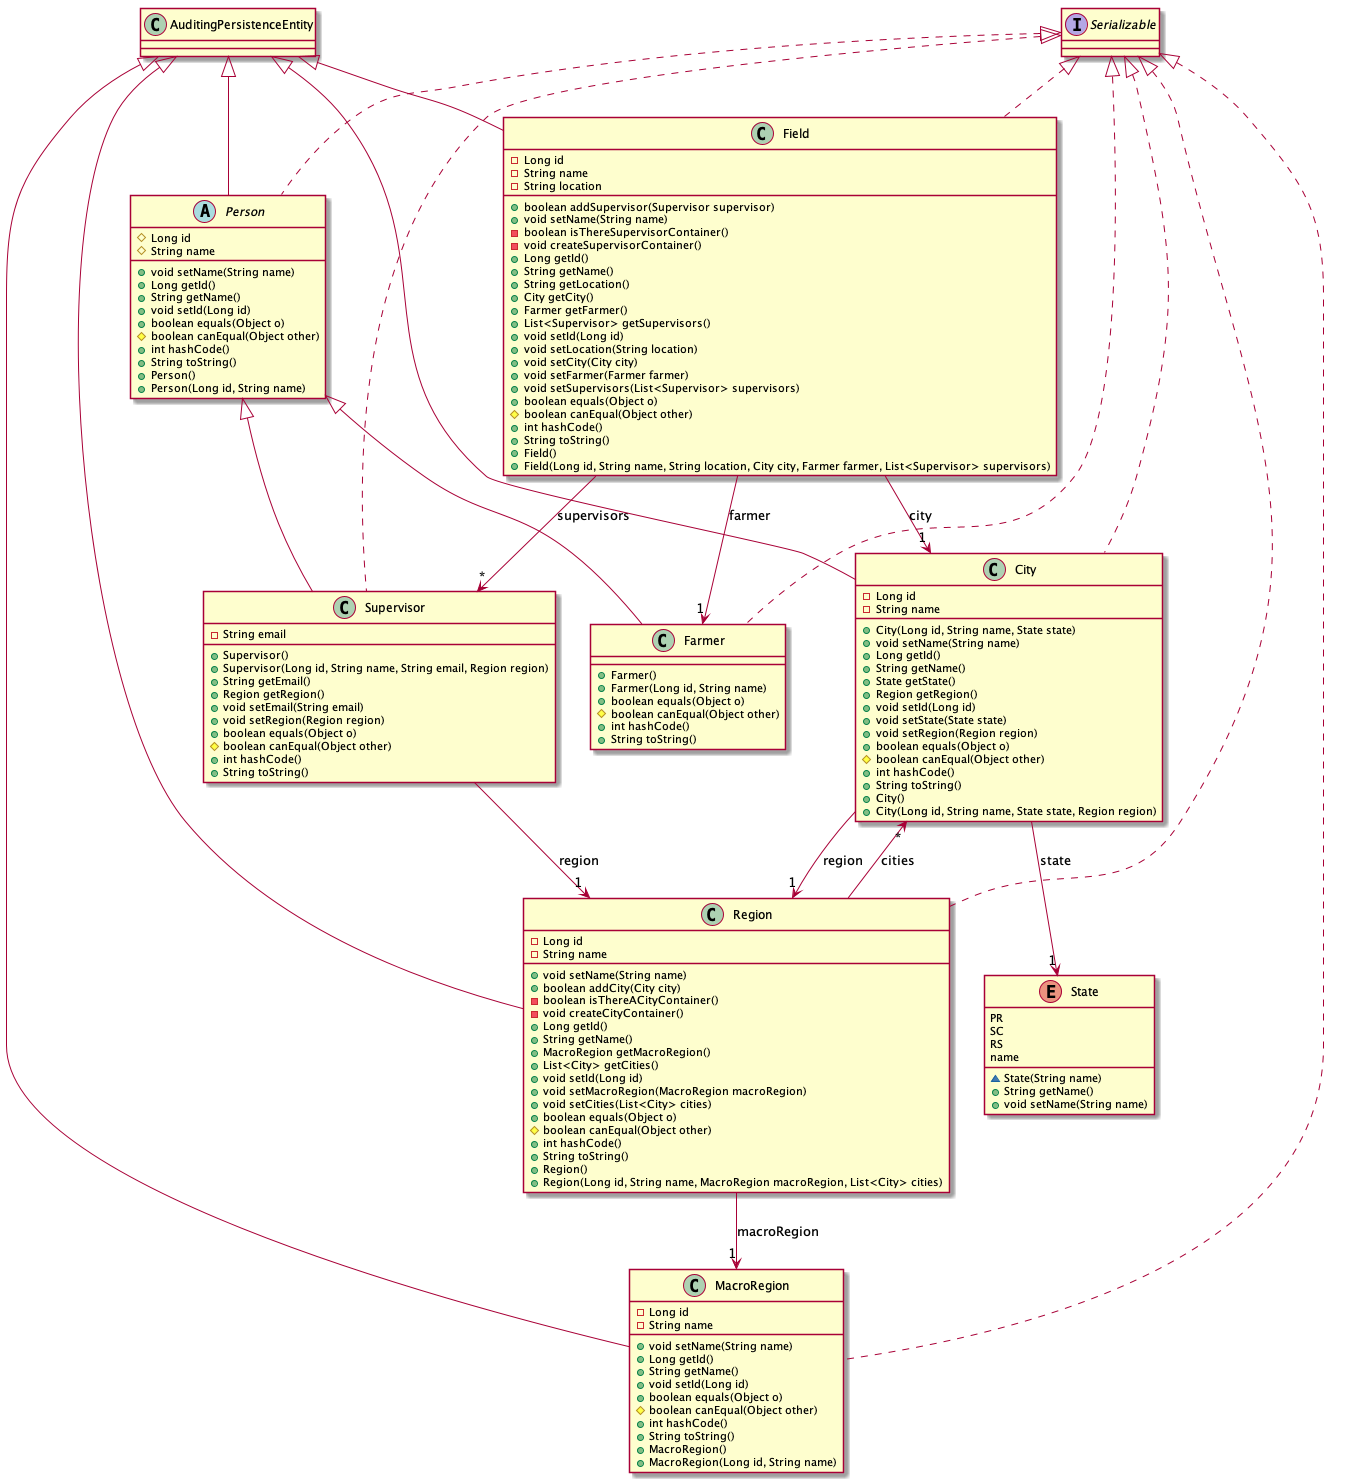
\includegraphics[scale=0.35]{dados/figuras/domain-base-classes.png}
	\caption{Diagrama de Classes Bases do Sistema.}
	FONTE: \cite[https:~//github.com/gabrielcostasilva/emater-mip-datacollection-app/tree/DDDLike/mip/src/main/resources/UMLDiagrams]{gabriel}
	\label{domain-base}
\end{figure}


\begin{landscape}
A FIGURA \ref{domain-survey} representa as classes relacionadas ao domínio das funcionalidades de pesquisa. No contexto da engenharia de software domínio de um sistema representa um conjunto de sistemas ou áreas que se comportam de forma similar.

\begin{figure}[h!]
	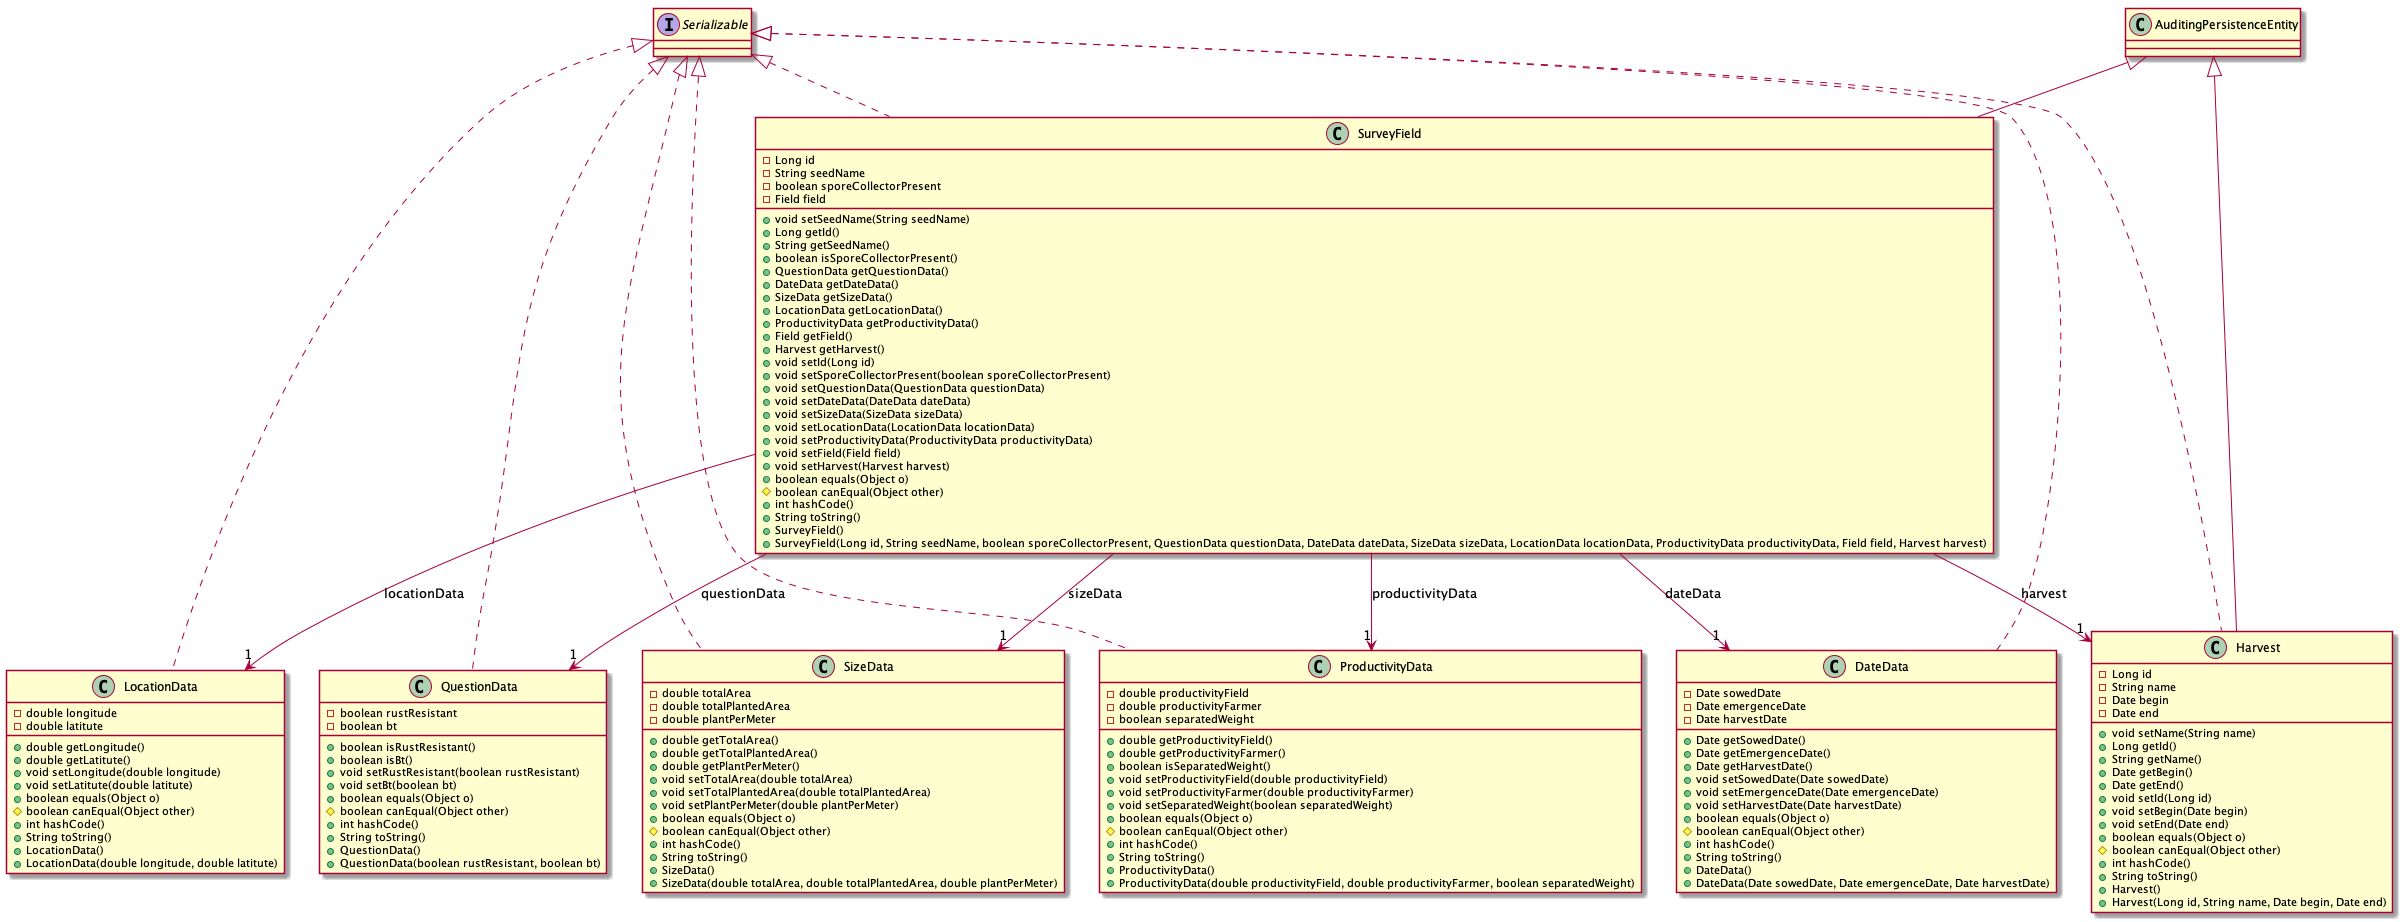
\includegraphics[scale=0.3]{dados/figuras/domain-survey-classes.png}
	\caption{Diagrama de Classes Domínio da Pesquisa.}
	FONTE: \cite[https:~//github.com/gabrielcostasilva/emater-mip-datacollection-app/tree/DDDLike/mip/src/main/resources/UMLDiagrams]{gabriel}
	\label{domain-survey}
\end{figure}
\end{landscape}



A FIGURA \ref{domain-pest} representa as classes relacionadas a coleta de dados sobre pragas. Funcionalidades de gerenciamento de pragas são apresentadas neste diagrama. 

\begin{figure}[h!]
	\centering
	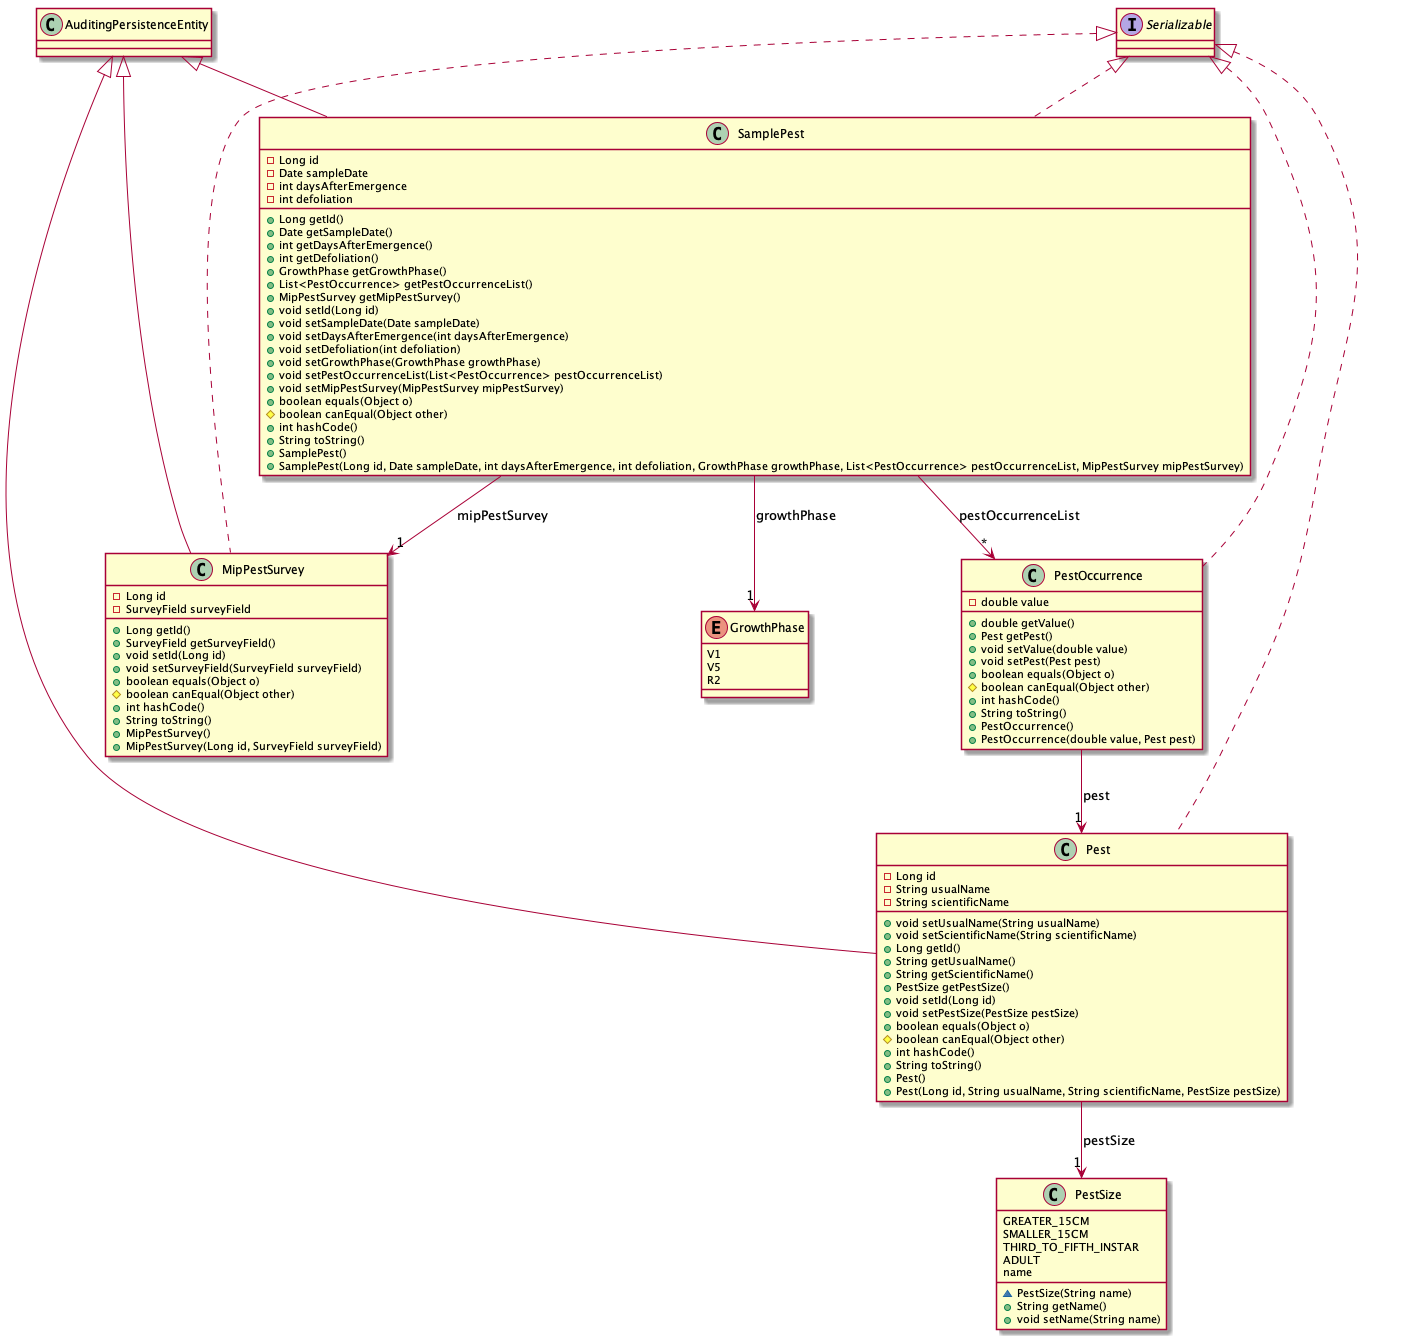
\includegraphics[scale=0.35]{dados/figuras/domain-mip-classes.png}
	\caption{Diagrama de Classes Gerenciamento de Pragas.} 
	FONTE: \cite[https:~//github.com/gabrielcostasilva/emater-mip-datacollection-app/tree/DDDLike/mip/src/main/resources/UMLDiagrams]{gabriel}
	\label{domain-pest}
\end{figure}



\section{TECNOLOGIA JAVA}

O Java é uma linguagem de programação e plataforma computacional orientada a objetos lançada pela primeira vez pela Sun Microsystems em 1995 e posteriormente adquirida pela ORACLE. Diferente das linguagens de programação convencionais, que são compiladas para código nativo o Java é compilada para um \textit{bytecode}\footnote{Conjunto de instruções projetada para execução eficiente por um interpretador de software. } que é interpretado por uma JVM \cite{Java}. A linguagem Java foi projetada para possuir portabilidade independente de plataforma, e segurança de rede, implementando restrições de execução.

\section{FERRAMENTAS}

A seguir, as ferramentas que serão utilizados no desenvolvimento dos
testes do sistema.

\subsection{JUnit}

O  \textit{JUnit} é um \textit{framework} para plataforma Java que possibilita a criação de classes de teste unitário. Por se tratar de uma ferramenta bastante difundida possui integração com diversas plataformas e IDEs. Além de tudo, ele é um projeto \textit{opensource}\footnote{Software de código aberto produzido de forma pública e colaborativa ou liberado sob uma licença na qual o detentor dos direitos autorais concede aos usuários os direitos para estudar, alterar e distribuir o software.} e permite que os testes sejam automatizados com apresentação de resultados. Os testes podem ser elaborados a partir dos requisitos do sistema ou casos de uso. 


Mais informações podem ser encontradas no capítulo 2 deste trabalho.

\subsection{Mockito}

O Mockito é um \textit{framework} de código aberto orientado a comportamento. Ele possibilita a simulação de comportamento de classes e interfaces facilitando a criação de testes que dependem de funcionalidades que ainda não foram implementadas. A ferramenta é bem difundida e possui integração com diferentes plataformas e IDEs. 

Mais informações podem ser encontradas no capítulo 2 deste trabalho.

\subsection{Spring Boot Test}

 Spring é um framework de código aberto, criado por Rod Johnson e possui o módulo de inicialização rápida. Spring Boot que é um projeto para facilitar o processo de configuração e publicação de aplicações \cite{spring}. O \textit{Spring Boot Test}  fornece suporte a testes de integração de forma fácil e simples. Através de anotações que o \textit{framework} disponibiliza é possível inicializar uma interface de conexão com o banco de dados permitindo a realização de testes de persistência e recuperação de dados.


Mais informações podem ser encontradas no capítulo 2 deste trabalho.

\subsection{IntelliJ IDEA}

O ambiente de desenvolvimento integrado IntelliJ IDEA, desenvolvido pela JetBrains é um programa  para desenvolvimento de \textit{software} em várias linguagens que suporta várias tecnologias e \textit{frameworks}. O Intellij possui um decompilador\footnote{Realiza a operação inversa de um compilador, transformando código objeto em código fonte.}, que permite debugar\footnote{Método para procurar um erro em um trecho de código.} o código interno de classes desenvolvidas e códigos externo de bibliotecas que não possuem fonte. Ele também conta com recursos de conexão a banco de dados o que permitem criar, alterar e excluir registros. Além de contar com a pesquisa rápida que permite a visualização e previsão de resultados, facilitando a interação com classes, bibliotecas e \textit{frameworks} \cite{intellij}.


\section{MÉTODO}

O sistema de Manejo Integrado de Pragas e Doenças deverá ser submetido a testes de unidade e integração. Os testes de unidade avaliarão isoladamente o banco de dados, as interfaces de comunicação, e todos os outros componentes do projeto. Os testes de integração testarão os componentes, previamente testados isoladamente, acoplados. O objetivo é identificar possíveis falhas nos acoplamentos. 


O processo de teste deve se basear em uma metodologia compatível com o processo de desenvolvimento e deve ser o guia básico para organizar a atividade de teste da aplicação. 


\subsection{Modelo 3P x 3E}

O modelo proposto é composto por diversas fases e etapas sendo duas em paralelo e quatro em sequência. As etapas em paralelo representam a preparação e o planejamento que devem estar presentes no projeto des de sua concepção e fornece suporte para as demais etapas do processo. Procedimentos iniciais representam a menor parte do processo, a maior parte do processo deve se dedicar as etapas de especificação, execução e entrega \cite{riosMoreira}. A FIGURA \ref{modelo3p3e} apresenta o modelo.


\begin{figure}[H]
	\centering
	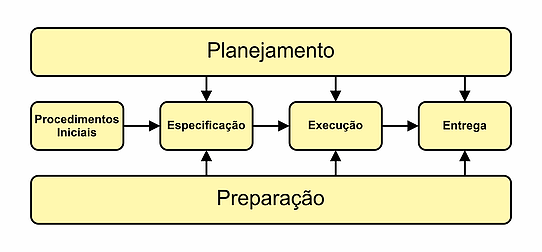
\includegraphics[scale=3.5]{dados/figuras/modelo3px3e.png}
	\caption{Modelo 3P x 3E do ciclo de vida do processo de teste.}FONTE: \cite{riosMoreira}
	\label{modelo3p3e}
\end{figure}



A primeira etapa “Procedimentos iniciais” propõe a análise e verificação dos requisitos para garantir que estes estejam completos e sem ambiguidades. Além disso o procedimento inicial deve conter as atividades que serão executadas ao longo de todo o desenvolvimento dos testes.


A segunda etapa de “Especificação” consiste em elaboração de casos de teste e elaboração de roteiros de teste. Deve-se retornar a esta etapa quando necessário pois novos requisitos podem surgir ou se alterarem.

A terceira etapa de “execução” se refere a etapa anterior de “Especificação”, os casos e roteiros de testes devem ser executados e seus resultados encontrados devem ser relatados.


 A quarta etapa “Entrega” se refere a finalização do processo de teste onde serão entregues os resultados obtidos e os artefatos gerados durante todo o processo.
 
 
As etapas de “Planejamento e Preparação” se dão ao longo de todo o projeto e são utilizadas de apoio, a preparação é basicamente responsável por preparar todo o ambiente de teste para que não haja obstáculos durante a execução, o planejamento é a atividade que permanece ativa durante todo o projeto para evitar desvios do objetivo principal.

\section{VALIDAÇÃO DO PROJETO}

% Esse é um teste\footnote{Esse é o exemplo de nota de rodaé.}.

Esta atividade se resume em avaliar se os artefatos entregues atendem com eficiência as metas propostas, além de apontar possíveis melhorias. Para cada requisito do sistema deve ser possível produzir um ou mais casos de testes de caixa-preta para verificar se o sistema cumpre o que foi projetado para fazer. Os testes definidos devem possuir um roteiro bem estruturado para validação do requisito, se não for possível a criação de um teste para um requisito será necessária uma melhor especificação deste requisito. Após os testes especificados estes serão executados por desenvolvedores e usuários para a validação do sistema. Ao final os testadores devem responder a um questionário fechado com perguntas pré-definidas. A partir do resultado do questionário serão levantados os pontos positivos e negativos do sistema, e possíveis melhorias podem ser acatadas.